\documentclass{report}\usepackage[]{graphicx}\usepackage[]{color}
%% maxwidth is the original width if it is less than linewidth
%% otherwise use linewidth (to make sure the graphics do not exceed the margin)
\makeatletter
\def\maxwidth{ %
  \ifdim\Gin@nat@width>\linewidth
    \linewidth
  \else
    \Gin@nat@width
  \fi
}
\makeatother

\definecolor{fgcolor}{rgb}{0.345, 0.345, 0.345}
\newcommand{\hlnum}[1]{\textcolor[rgb]{0.686,0.059,0.569}{#1}}%
\newcommand{\hlstr}[1]{\textcolor[rgb]{0.192,0.494,0.8}{#1}}%
\newcommand{\hlcom}[1]{\textcolor[rgb]{0.678,0.584,0.686}{\textit{#1}}}%
\newcommand{\hlopt}[1]{\textcolor[rgb]{0,0,0}{#1}}%
\newcommand{\hlstd}[1]{\textcolor[rgb]{0.345,0.345,0.345}{#1}}%
\newcommand{\hlkwa}[1]{\textcolor[rgb]{0.161,0.373,0.58}{\textbf{#1}}}%
\newcommand{\hlkwb}[1]{\textcolor[rgb]{0.69,0.353,0.396}{#1}}%
\newcommand{\hlkwc}[1]{\textcolor[rgb]{0.333,0.667,0.333}{#1}}%
\newcommand{\hlkwd}[1]{\textcolor[rgb]{0.737,0.353,0.396}{\textbf{#1}}}%

\usepackage{framed}
\makeatletter
\newenvironment{kframe}{%
 \def\at@end@of@kframe{}%
 \ifinner\ifhmode%
  \def\at@end@of@kframe{\end{minipage}}%
  \begin{minipage}{\columnwidth}%
 \fi\fi%
 \def\FrameCommand##1{\hskip\@totalleftmargin \hskip-\fboxsep
 \colorbox{shadecolor}{##1}\hskip-\fboxsep
     % There is no \\@totalrightmargin, so:
     \hskip-\linewidth \hskip-\@totalleftmargin \hskip\columnwidth}%
 \MakeFramed {\advance\hsize-\width
   \@totalleftmargin\z@ \linewidth\hsize
   \@setminipage}}%
 {\par\unskip\endMakeFramed%
 \at@end@of@kframe}
\makeatother

\definecolor{shadecolor}{rgb}{.97, .97, .97}
\definecolor{messagecolor}{rgb}{0, 0, 0}
\definecolor{warningcolor}{rgb}{1, 0, 1}
\definecolor{errorcolor}{rgb}{1, 0, 0}
\newenvironment{knitrout}{}{} % an empty environment to be redefined in TeX

\usepackage{alltt}
\usepackage{geometry}
\geometry{a4paper,textwidth=15.92cm,textheight=24.62cm}
\usepackage{verbatim}
\usepackage{rotating}
\usepackage{lscape}
\usepackage{hyperref}
\usepackage[T1]{fontenc}
%\usepackage[nodayofweek]{datetime}
\usepackage[ddmmyy]{datetime}
\usepackage{enumitem}
\usepackage{setspace}
\usepackage{graphicx,wrapfig,lipsum}
\usepackage{fancyhdr}
\usepackage{longtable}
\usepackage{caption}

\makeatletter
\newcommand{\verbatimfont}[1]{\def\verbatim@font{#1}}%
\makeatother

% following to define a new section style that takes less space
\makeatletter % make "at" ("@") letter, important for the code that follows
\renewcommand\chapter{\@startsection%
{chapter}{1}{0pt}%name, level, indent
{-\baselineskip}%beforeskip
{0.2\baselineskip}%afterskip
{\raggedright\bf}}%
\makeatother

\makeatletter
\renewcommand\section{\@startsection%
{section}{2}{0pt}%name, level, indent
{-\baselineskip}%beforeskip
{0.2\baselineskip}%afterskip
{\raggedright\bf}}%
\makeatother

\setlength{\parskip}{1em}
\renewcommand*\contentsname{Table of contents}

\newcommand{\MONTH}{%
  \ifcase\the\month
  \or January
  \or February
  \or March
  \or April
  \or May
  \or June
  \or July
  \or August
  \or September
  \or October
  \or November
  \or December
  \fi}

\renewcommand{\dateseparator}{}

\definecolor{green}{rgb}{0,0.8,0}
\definecolor{gray}{rgb}{0.5,0.5,0.5}

\pagestyle{fancy}
\fancyhf{}
\fancyhead[L]{\textcolor{gray}{THE NATURE CONSERVANCY INDONESIA FISHERIES CONSERVATION PROGRAM \\ AR\_ASSESSMENTGUIDE\_{\today}}}
\rfoot{\thepage}
\IfFileExists{upquote.sty}{\usepackage{upquote}}{}
\begin{document}
% use "echo=False" to remove R code from the output


\newgeometry{left=1cm,top=1cm,right=1cm,bottom=1cm}
\begin{titlepage}
\begin{flushleft}
	\textsf{Report Code: AR\_GROUPER\_{\today}}
\end{flushleft}

\vspace*{2cm}
\begin{flushright}
        {\Large\textsf{Length-Based Assessment of Data-Poor Multi-Species Deep Grouper Fisheries in 
        \\[0.2cm] Fisheries Management Areas (WPP) 573, 712, 713, 714, 715 \& 718 in Indonesia}}\\[0.2cm]
        \rule{\linewidth}{0.5mm}
        \textsf{DRAFT - NOT FOR DISTRIBUTION. TNC-IFCP Technical Paper}\\[2cm]
        \textsf{Peter J. Mous, Jos S. Pet\\[1cm]
        {\MakeUppercase{\MONTH}} {\the\day}, {\the\year}}
\end{flushright}

\begin{center}
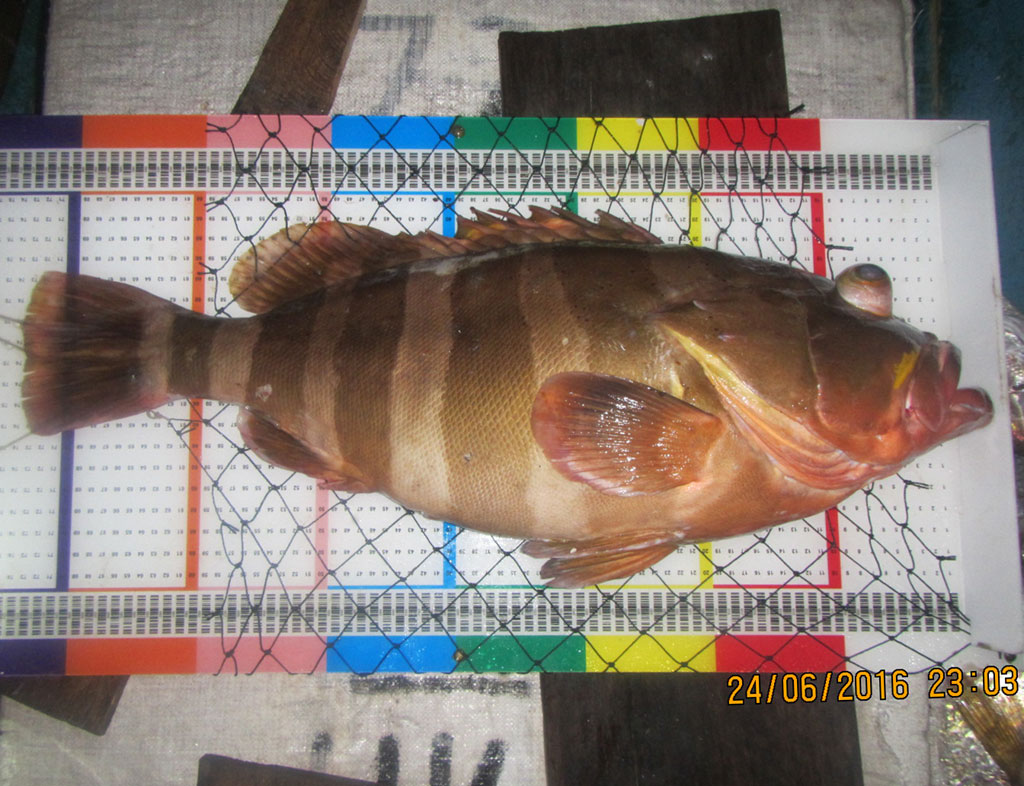
\includegraphics[width=.9\linewidth]{/root/R-project/IFishGrouper/Images/cover_ifish_grouper.jpg}
\end{center}

\vfill

\noindent
\begin{minipage}[b]{\linewidth}
\noindent
\centering
$\vcenter{\hbox{
\includegraphics[width=.3\linewidth]{/root/R-project/IFishGrouper/Images/usaid.png}}}$
\hfill
$\vcenter{\hbox{
\includegraphics[width=.3\linewidth]{/root/R-project/IFishGrouper/Images/tnc.png}}}$
\hfill
$\vcenter{\hbox{
\includegraphics[width=.3\linewidth]{/root/R-project/IFishGrouper/Images/pnci.png}}}$
\end{minipage}
\end{titlepage}
\restoregeometry

\vspace*{\fill}
\begin{sffamily}
\noindent\large For inquiries, please contact Dr. Peter Mous at pmous@tnc.org or Dr. Jos Pet at pet.jos@gmail.com\\
\end{sffamily}

\noindent
\fbox{\begin{minipage}[b]{\linewidth}
\begin{sffamily}
\begin{spacing}{0.4}
\textbf{The Nature Conservancy Indonesia Fisheries Conservation Program}\\[0.1cm]
Jl. Pura Segara, Pelabuhan Raya Benoa\\
Denpasar 3012\\
Bali, Indonesia\\
Ph. +62-361-244524, fax +62-361-244532\\[1cm]

\textbf{People and Nature Consulting International}\\[0.1cm]
Grahalia Tiying Gading 18, Suite 2\\
Jalan Tukad Pancoran, Panjer\\
Denpasar 80225
Bali, Indonesia\\
Ph. +62-361-257246\\
\end{spacing}
\end{sffamily}
\end{minipage}}
\clearpage

\tableofcontents

\clearpage
\newpage

\large

\chapter{Introduction}
This report presents a length-based assessment of the multi-species deep slope fisheries targeting mostly snappers, groupers and emperors, at depths ranging from 50 to 500 meters, in fisheries management areas (WPP) 714 and 715 in eastern Indonesia. These WPPs cover the Maluku, Seram, Banda and Flores Seas and they were combined as a single area for analysis, as the border between WPP 714 and WPP 715 cuts through the middle of the fishing grounds. Drop line and mini long line vessels fish on both sides of this border sometimes even within a single fishing trip. Also in terms of habitat and ecology of the target species the 2 WPPs covered in this report are very similar and completely connected. Fishing grounds for snappers, groupers, emperors and other target species in this region include deep slopes along the many islands as well as seamounts and other deep structures which are characteristic for this area.

Several fleets from this region contributed data to the current assessment, including a medium scale drop line fishery based in Kema (20 boats), North Sulawesi, and a small scale mini long line fishery based in the Banggai and Sula Islands on the border of the Maluku and Banda Seas. In addition, data were used from fleets originating from outside the region (e.g. Bali, Probolinggo, Kupang) but operating inside WPP 714 and/or WPP715. Fishing grounds for the small scale mini long line fleet are concentrated near the home islands near the center of our area of interest, whereas the medium scale drop liners from Kema make trips to locations up to 1,000 kilometers away from their port, to all corners of this region.

Kema based vessels make up to about 10 trips a year, landing around 4 tons of mixed snapper, grouper and emperor for each trip or up to about 40 tons per vessel per year. The drop line fishery is an active vertical hook and line fishery operating at depths from 50 to 500 meters, whereas long lines are set horizontally along the bottom at depths ranging from 50 to 150 meters. This report analyzes length frequencies of the 50 species of fish that were the most abundant in the combined drop and long line fisheries operating in WPP 714 and WPP 715. For a complete overview of the species composition please refer to the ID guide prepared for these fisheries:

\textbf{CLICK: }\href{http://72.14.187.103:8080/ifish/pub/TNC_FishID.pdf}{Link to on-line E-Book Species ID Guide}

For further background on species life history characteristics, and data-poor length based assessment methods, as applied in this report, please refer to the assessment guide that was separately prepared for these fisheries:

\textbf{CLICK: }\href{http://72.14.187.103:8080/ifish/pub/DeepSlopeSpeciesAssessmentTool.pdf}{Link to on-line E-Book Assessment Guide with Biological Information}

Data in this report represent complete catches by small and medium scale vessels from the above described fleets. All fish captured were photographed on measuring boards by fishing crew participating in our Crew Operated Data Recording System or CODRS. Images were analyzed by project staff to generate the species specific length frequency distributions of the catches which served as the input for our length based assessment of this fishery.

\begin{center}
\graphicspath{{/root/R-project/IFishSnapperWPP714_715/Images/}}
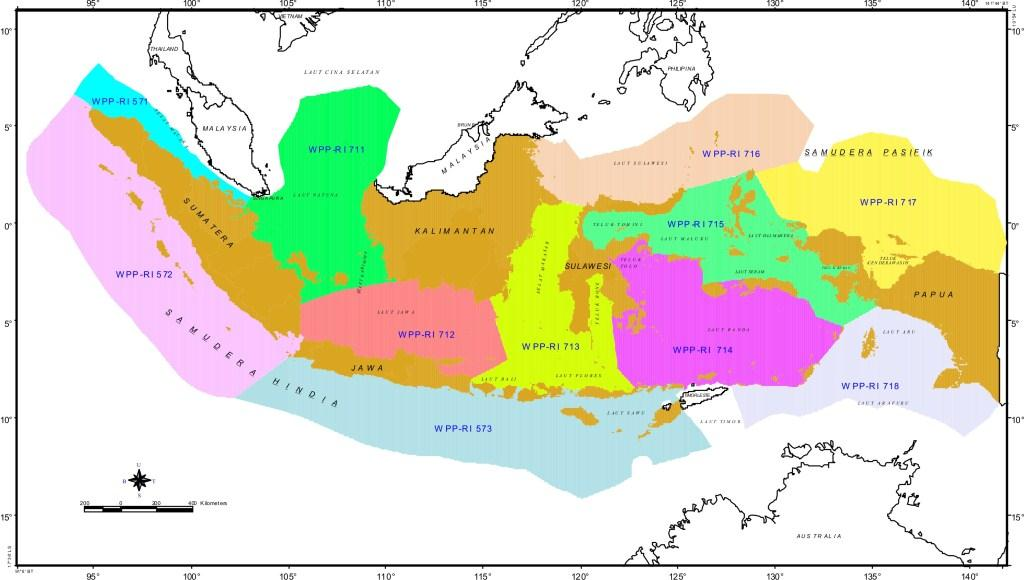
\includegraphics[scale=1.8]{wpp-indonesia.jpg}

Figure 1. Fisheries Management Areas (WPP) in Indonesian marine waters.
\end{center}

\begin{center}
\graphicspath{{/root/R-project/IFishSnapperWPP714_715/Images/}}
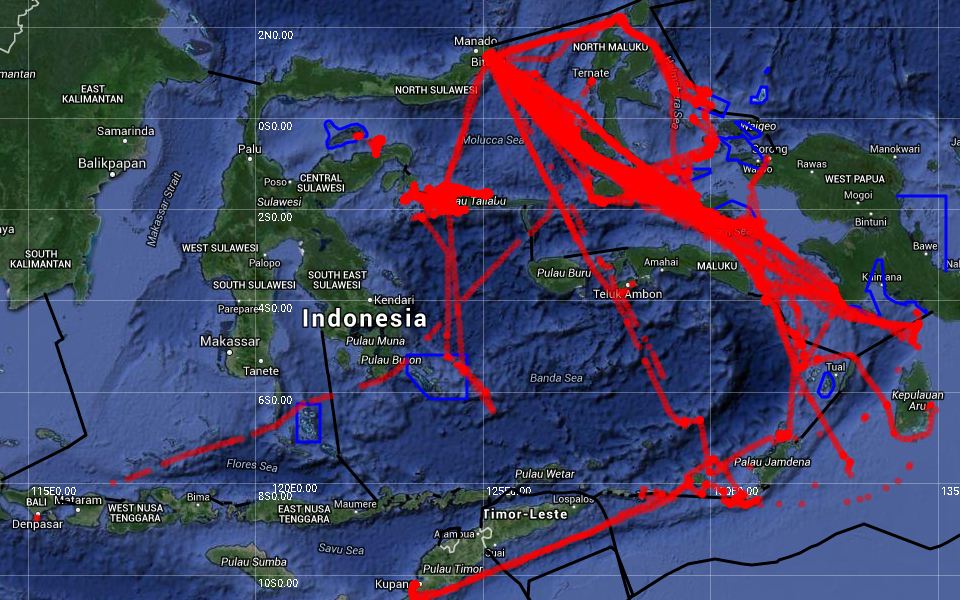
\includegraphics[scale=0.6]{SpotTrace-AreaC-Satellite.jpg}

Figure 2. Map with fishing ground bathymetry and tracks (in red) of snapper fishing trips into WPP 714 and 715. Black lines are WPP boundaries, blue lines are MPA boundaries. This figure mainly represents fleets from Kema (near Manado) and the Banggai / Sula Islands.
\end{center}

\clearpage
\newpage

\chapter{Estimating Values of Key Life History Parameters}
\section{Life History Parameter Values and Invariables}
With the exception of \textit{E. coruscans}, some of which (but not all) have a greatly elongated upper lobe of the tail fin, all length-based information in this document relates to Total Length (\textbf{TL}) of the fish, as measured from the tip of the snout to the longest tip of the tail fin. For \textit{E. coruscans} we have used the tip of the lower lobe of the tail fin to measure total length. For cross checking of values in the literature on Fork Length (\textbf{FL}), we have used literature information on \textbf{TL/FL} conversion factors by species.

Our length-based assessment approach is based on four life-history characteristics or parameters; \textbf{Lmax, Linf, Lopt, and Lmat} (explained below). Published values for these characteristics are available for some species but lacking for many. Values for specific species vary between publications and are often unreliable due to misidentifications and/or sampling bias issues (small samples which lack the larger specimen). We therefore used an estimation procedure based on life history invariable values, which only requires accurate knowledge on Lmax, the maximum attainable size of each species, in combination with family-specific relationships (life history invariables) between Lmax and each of the other parameters. Meta-analysis results from the literature are available to obtain values for life history invariables for various ranges of species. This approach is gaining increasing interest in the scientific community (e.g. Nadon and Ault, 2016) and provides the breakthrough allowing accurate length based assessments of data poor fisheries.

\section{Maximum Total Length}
\textbf{Maximum attainable total length (Lmax)} by species was estimated from a range of information sources, including published values, lengths of trophy fish, anecdotal information and an ever increasing amount of data from our fisheries monitoring work. Published values of maximum size were treated carefully as there are many issues with species identification, while under-estimation of Lmax is common in many publications that look only at small samples from intensively fished stocks.

For some species larger maximum sizes are attained at greater latitudes in cooler waters. When analyzing information from literature or images from the internet, we included only sizes of fish that were observed at latitudes within or close to the range covered by Indonesian fishing grounds. Maximum attainable total length in this document refers to maximum attainable total lengths at latitudes overlapping with or close to those of Indonesian fishing grounds.

By early 2017 our Crew Operated Data Recording System (CODRS) had produced over a quarter million images of the top 100 most abundant species from deep slope fisheries catches. With this huge sample size we were able to determine the sizes of the very largest specimen caught of each species, and determine their ID from CODRS images. For several species we found fish that were larger than previously reported for our region. In some other cases we had to decide on values for Lmax which were below sizes previously reported, mainly when we could not obtain confirmation on correct species ID for values presented in literature or on line. For many species we were able to verify estimates based on reliable information from nearby Australian fishing grounds or we obtained CODRS images proving maximum sizes to be obtained above what was previously reported.

\section{Asymptotic Length}
Our next life history characteristic, the ``\textbf{asymptotic length}'' (\textbf{Linf}), is defined here as the mean length in a cohort of very old fish (a cohort of infinite age). As such it is by definition smaller than the maximum length obtained within the population of a specific species. This asymptotic length, or the mean length at infinite age, is one of the growth parameters in the well known Von Bertalanffy growth equation. Without further exploring that equation, it is important to remember that we define Linf here as the mean length in the oldest cohort in the population. This asymptotic length of each species is an important parameter in fisheries assessment methods and management decision support models.

We have extensively used literature information and sometimes found under-estimation of Linf for target species that are heavily fished, probably due to the limited size range in the catch. Under-estimation due to misidentification of species also occurs in the literature. Over-estimation was also found, possibly again due to misidentification or due to other issues with input data used to estimate Linf. As a general rule though, as confirmed from data in published meta-analysis, we found that Linf could very well be estimated as 90\% of the maximum length, Lmax (e.g. Nadon and Ault, 2016).

A rule of thumb relationship ``\textbf{Linf =  0.9 * Lmax}'' can be explained by Lmax being the largest fish we observe, at about 1 standard deviation longer than Linf, in cohorts of fish with length frequencies that have a standard deviation of about 10\% of the mean length. We could assume that in general we do not get to observe the very largest fish in the population, as that really is the needle in the oceanic hay stack, and, probably more importantly, hardly any fish in this day and age actually survives to reach its potential maximum size. This estimation method (Linf =  0.9 * Lmax) was applied by us in this guide, to ensure we have realistic parameter values for all species even in our data-poor environment.

\section{Length at Maturation}
The  value of Linf (above) is important in the estimation of values of additional length-based life history characteristics for each target species, like the \textbf{length at maturation} (\textbf{Lmat}). Lmat is defined here as the smallest length class at which 50\% of the individuals (in that length class) are mature. Size at maturity is a particularly important parameter used to assess and evaluate the impact of fishing mortality on the spawning stock and to determine levels of optimum fishery yield.

Information on length at maturation was collected from a wide variety of sources for the target species in this guide. General trends were found for various families including those containing the most important target species, starting with the Lutjanidae (snappers). An important characteristic of snapper reproductive biology is that they do not change sex during their life (whereas several other families of fish do, see below). Sexual dimorphism is rare in snappers, only reported for coloration in two species of the genus Pristipomoides from the Indo-Pacific.

An important meta-analysis of all available information on life history parameters for Lutjanidae was published by Martinez-Andrade in 2003. This researcher developed a data base with parameter values for a wide range of species and collected information on relationships between the various parameters to make estimates where values were missing. For example for the sub-family of Lutjaninae (snappers) a strong correlation between Lmat and Linf was found from the meta-analysis and Lmat was estimated for these species by Martinez-Andrade from Lmat = 0.52 * Linf (Figure 1).

\begin{center}
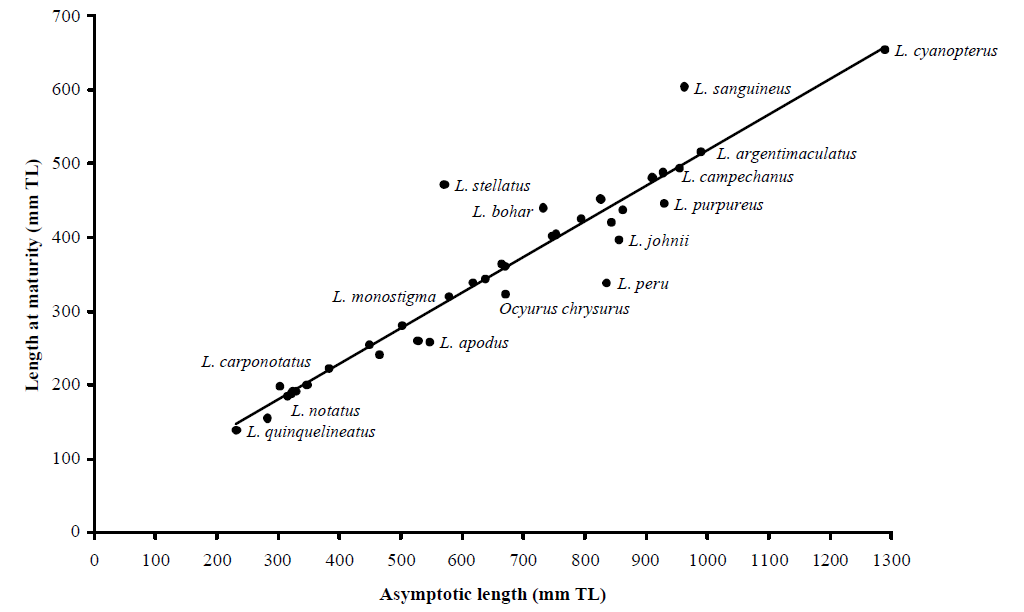
\includegraphics[width=1.1\linewidth]{/root/R-project/IFishAssessmentGuide/Images/LengthMaturity_vs_AsymptoticLength.png}
\end{center}
\textbf{Figure 1.} Length at maturity vs. asymptotic length in the family of Lutjanidae.

Over the decade after Martinez-Andrade published the relationship between Lmat and Linf for a wide range of snappers, small and large, shallow and deep water species, a lot more work was done on species identification and much more information has become available for deep water snappers. This enabled Newman and others (2016) to further refine the relationship for deep water snappers as \textbf{Lmat = 0.59*Linf}. As we are analyzing deep slope fisheries at depths below 50 meters in our program, we have adopted this life history invariable value and in this guide we use the general assumption that the \textbf{snappers targeted by our deep slope fisheries mature at about 59\% of their asymptotic length}. This assumption was verified species by species, using a range of information sources, and was shown to hold for those species in our fisheries, for which reliable direct information on maturation was available.

Epinephelidae (groupers) in general mature initially as females and later in life change sex to males. This explains certain characteristics of grouper populations. Males tend to be larger on the average than females and there is usually an overall sex ratio in favor of females. There is some overlap in size distributions between males and females in most groupers, suggesting that sex change can occur over a size range rather than occurs at a very narrow size class. Size at sex change may be partly influenced by sex ratio in the population and sex change from female to male may occur at smaller sizes when larger males are rare or absent from the population.

After looking at information on maturation for a range of species of deep water groupers we concur with Newman and others (2016) that \textbf{``deep water'' groupers mature as females at a size around 46\% of Linf}. We define deep water groupers here as those species of Epinephelidae which commonly occur in deep slope fisheries catches, from waters deeper than 50 meters. We define Lmat in groupers as the female maturation size which is estimated from \textbf{Lmat = 0.46*Linf}. For most groupers sex change from female to male seems to start at around 1.33*Lmat (1.33 times size at female maturation), after the cohort has reached maximum biomass and therewith maximum fecundity. It makes evolutionary sense that sex change from female to male would not start earlier.
 
Many Lethrinids (emperors) can undergo sex change from female to male. But not all individuals seem to follow this pattern and both sexes are found over a range of sizes above the size of first maturity. Some species, like spangled emperor, sometimes change sex from female to male before they reach maturity (if they are going to change sex at all) and females and males can mature at around the same length. In general there is considerable overlap in size distributions between males and females in most emperor species, and for purposes of emperor fisheries management, it is more meaningful to define a length at maturity by species only, rather than separately for the sexes. \textbf{In general emperors seem to be maturing at about 50\% of their asymptotic length}. We have used \textbf{Lmat = 0.5*Linf} on the basis of a review of a range of information sources and applied this for our estimates of size at maturity in emperors. In most if not all cases, this general assumption showed good overlap with published ranges for maturity in emperors.

From sketchy available information we extrapolated that for most other species in our target list our best possible estimate for length at maturation would be around 50\% of the asymptotic length, as found also for emperors. Starting from the meta-analysis of snappers by Martinez-Andrade (2003) right through a range of other information sources on length at maturation, a constant of about 50\% of Linf was found to be our best estimator for length at maturation in most of our target species, except for the deep water snappers and groupers. This estimator is also confirmed by a relationship of Lmat = 0.461 * Lmax reported from another meta-analysis by Binohlan and Froese (2009). One exception to this general rule may exist for larger Carangids which are also found in the catches of the deep slope fisheries. Reliable and precise information however is scarce and we did not find enough detailed information to deviate from the general 50\% rule for carangids either.

\begin{center}
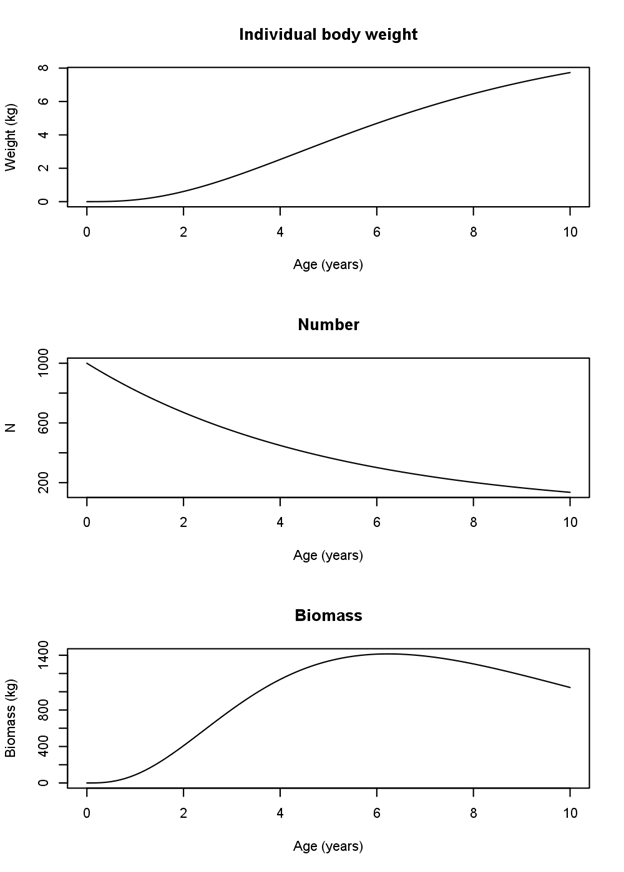
\includegraphics[width=.9\linewidth]{/root/R-project/IFishAssessmentGuide/Images/Figure-2.png}
\end{center}
\textbf{Figure 2.} The biomass of a cohort of (imaginary) fish in an un-fished situation reaches its maximum at an age (and at the related size of the fish in the cohort) where growth of individuals has slowed down to the point that it does not make up anymore for biomass loss through natural mortality.

\section{Optimum Harvest Size}
The final length-based life history characteristic that we will be using in our length-based assessment method is the \textbf{length class with the highest biomass in an un-fished population (Lopt)}. It is at this length (and corresponding age) that the biomass expressed as the number of survivors (in an un-fished cohort) multiplied with their average weight reaches a maximum (Figure 2). A fishery will obtain the maximum possible yield if it catches fish mainly around this size. Thus, fisheries managers should strive to adjust the mean length (or median length) in their catch towards this value.

Reproductive output in terms of total number of eggs (fecundity) is also optimized at this length (Lopt), where the biomass of the un-fished cohort is maximized. So also from a perspective of maximizing recruitment to the fishery, managers would strive to focus their fishery on size classes around Lopt (well beyond Lmat). And for sex-changing groupers it is important that cohorts are not decimated before sufficient individuals have changed sex from female to male, a process which begins around the size of Lopt.

Lopt can be estimated from empirical relationships between Lopt and Lmat. Lopt for catching a range of demersal fish species could be estimated as 1.33 * the length where 50\% of the fish are mature (\textbf{Lopt = 1.33 * Lmat}), based on the median values for this life history invariable (Lmat/Lopt = 0.75) over a range of demersal species (Cope and Punt, 2009). We have chosen to use this estimator of 1.33*Lmat for Lopt as the Cope and Punt (2009) study seemed to be one of the best researched situations in terms of estimating Lopt for a group of species with comparable biology and life history.


\clearpage
\newpage

\chapter{A Simple Length-Based Assessment Tool}
\input{/root/R-project/IFishAssessmentGuide/Texs/3_length_based.tex}

\clearpage
\newpage
\setlength{\tabcolsep}{5pt}
\captionsetup{width=1\textwidth, justification=centering}
\setlength{\LTpost}{0pt}
% latex table generated in R 3.2.2 by xtable 1.7-4 package
% Sat Jan 21 12:25:23 2017
{\small
\begin{longtable}{ccccccccc}
\caption{Ranking and Sample Sizes of 50 Most Abundant Species \\in Indonesian Deep Water Hook-And-Line Fisheries} \\ 
  \hline
Rank & ID\# & Species & Nsample & Lx-codrs & Lmax & Linf & Lopt & Lm50 \\ 
  \hline
1 & 7 & Pristipomoides multidens & 63893 & 90 & 100 & 90 & 71 & 53 \\ 
  2 & 8 & Pristipomoides typus & 30362 & 662 & 85 & 77 & 60 & 45 \\ 
  3 & 45 & Epinephelus areolatus & 25381 & 49 & 50 & 45 & 28 & 21 \\ 
  4 & 9 & Pristipomoides filamentosus & 23752 & 86 & 90 & 81 & 64 & 48 \\ 
  5 & 1 & Aphareus rutilans & 14082 & 112 & 125 & 113 & 88 & 66 \\ 
  6 & 34 & Paracaesio kusakarii & 13597 & 80 & 85 & 77 & 60 & 45 \\ 
  7 & 18 & Lutjanus malabaricus & 12746 & 90 & 100 & 90 & 71 & 53 \\ 
  8 & 4 & Etelis sp. & 10727 & 120 & 130 & 117 & 92 & 69 \\ 
  9 & 10 & Pristipomoides sieboldii & 10008 & 55 & 60 & 54 & 42 & 32 \\ 
  10 & 23 & Pinjalo lewisi & 8916 & 61 & 55 & 50 & 39 & 29 \\ 
  11 & 22 & Lutjanus erythropterus & 7724 & 69 & 70 & 63 & 49 & 37 \\ 
  12 & 6 & Etelis coruscans & 7437 & 120 & 130 & 117 & 92 & 69 \\ 
  13 & 20 & Lutjanus timorensis & 6440 & 60 & 60 & 54 & 42 & 32 \\ 
  14 & 71 & Gymnocranius grandoculis & 5758 & 74 & 80 & 72 & 48 & 36 \\ 
  15 & 27 & Lutjanus vitta & 5134 & 43 & 45 & 41 & 32 & 24 \\ 
  16 & 70 & Wattsia mossambica & 4345 & 59 & 60 & 54 & 36 & 27 \\ 
  17 & 35 & Paracaesio stonei & 4086 & 67 & 70 & 63 & 49 & 37 \\ 
  18 & 19 & Lutjanus sebae & 3549 & 96 & 100 & 90 & 71 & 53 \\ 
  19 & 5 & Etelis radiosus & 2274 & 103 & 105 & 95 & 74 & 56 \\ 
  20 & 43 & Epinephelus morrhua & 2049 & 71 & 75 & 68 & 41 & 31 \\ 
  21 & 32 & Paracaesio gonzalesi & 1903 & 51 & 55 & 50 & 39 & 29 \\ 
  22 & 39 & Cephalopholis sonnerati & 1861 & 52 & 55 & 50 & 30 & 23 \\ 
  23 & 51 & Epinephelus chlorostigma & 1842 & 63 & 75 & 68 & 41 & 31 \\ 
  24 & 2 & Aprion virescens & 1782 & 107 & 110 & 99 & 78 & 58 \\ 
  25 & 88 & Glaucosoma buergeri & 1579 & 67 & 70 & 63 & 42 & 32 \\ 
  26 & 84 & Seriola rivoliana & 1456 & 120 & 135 & 122 & 81 & 61 \\ 
  27 & 16 & Lutjanus argentimaculatus & 1436 & 95 & 100 & 90 & 71 & 53 \\ 
  28 & 85 & Erythrocles schlegelii & 1394 & 90 & 90 & 81 & 54 & 41 \\ 
  29 & 68 & Lethrinus amboinensis & 1175 & 56 & 60 & 54 & 36 & 27 \\ 
  30 & 33 & Paracaesio xanthura & 1099 & 49 & 50 & 45 & 35 & 27 \\ 
  31 & 17 & Lutjanus bohar & 1099 & 88 & 90 & 81 & 64 & 48 \\ 
  32 & 67 & Lethrinus olivaceus & 1059 & 97 & 100 & 90 & 60 & 45 \\ 
  33 & 21 & Lutjanus gibbus & 954 & 48 & 50 & 45 & 35 & 27 \\ 
  34 & 90 & Diagramma pictum & 900 & 81 & 85 & 77 & 51 & 38 \\ 
  35 & 76 & Carangoides chrysophrys & 822 & 80 & 80 & 72 & 48 & 36 \\ 
  36 & 80 & Caranx sexfasciatus & 808 & 82 & 85 & 77 & 51 & 38 \\ 
  37 & 65 & Lethrinus lentjan & 793 & 50 & 55 & 50 & 33 & 25 \\ 
  38 & 58 & Epinephelus amblycephalus & 787 & 78 & 80 & 72 & 44 & 33 \\ 
  39 & 72 & Gymnocranius griseus & 783 & 44 & 45 & 41 & 27 & 20 \\ 
  40 & 31 & Symphorus nematophorus & 775 & 97 & 100 & 90 & 71 & 53 \\ 
  41 & 30 & Lipocheilus carnolabrum & 764 & 73 & 75 & 68 & 53 & 40 \\ 
  42 & 91 & Cookeolus japonicus & 744 & 62 & 65 & 59 & 39 & 29 \\ 
  43 & 87 & Dentex carpenteri & 717 & 42 & 45 & 41 & 27 & 20 \\ 
  44 & 86 & Argyrops spinifer & 709 & 50 & 55 & 50 & 33 & 25 \\ 
  45 & 53 & Epinephelus heniochus & 623 & 56 & 60 & 54 & 33 & 25 \\ 
  46 & 82 & Elagatis bipinnulata & 597 & 104 & 110 & 99 & 66 & 50 \\ 
  47 & 77 & Carangoides gymnostethus & 533 & 84 & 90 & 81 & 54 & 41 \\ 
  48 & 14 & Pristipomoides flavipinnis & 515 & 54 & 60 & 54 & 42 & 32 \\ 
  49 & 61 & Plectropomus leopardus & 506 & 72 & 80 & 72 & 44 & 33 \\ 
  50 & 81 & Caranx tille & 502 & 88 & 90 & 81 & 54 & 41 \\ 
   \hline
\hline
\end{longtable}
}
 
\noindent{\small{\textbf{Nsample} is total sample including SWMS and CODRS data (mostly CODRS).
\textbf{Lx-codrs} = Largest specimen with verifiable ID and size from CODRS photo.
\textbf{Lmax} = maximum attainable total length at Indonesian lattitudes.
\textbf{Linf} = 0.9 * Lmax (with 10\% dispersion around mean size in cohort).
\textbf{Lm50} = Size at 50\% maturity.
\textbf{Lm50} = 0.59 * Linf for deep water lutjanidae (Newman et al., 2016).
\textbf{Lm50} = 0.46 * Linf for deep water Epinephelidae (Newman et al., 2016).
\textbf{Lm50} = 0.5 * Linf for Other Species (pooled literature).
\textbf{Lopt} = 1.33 * Lmat for range of demersals (Cope and Punt, 2009). All sizes in Total Length.}}
\clearpage
\newpage

\clearpage
\newpage

\chapter{Plotting Results From Length-Based Assessments}
\input{/root/R-project/IFishAssessmentGuide/Texs/4_plotting_results.tex}

\clearpage
\newpage

\chapter{Evaluating Results From Length-Based Assessments}
When looking at results from length-based assessments, we do need to be careful with conclusions, and consider the ecology and dynamics in all of the fisheries targeting the species under assessment, in all of the habitats utilized by all of the life stages of these species. Snappers for example, like most of our other target species, have pelagic eggs and larvae. The larval pelagic stage lasts for 4 to 6 weeks, when larvae are between 1 and 2 cm long. Eggs and larvae can be displaced over great distances, and pre-settlers actively swim in specific directions, and towards specific habitats, during this time. At the end of their pelagic migration, juvenile snappers settle on nursery grounds.

After settlement, juveniles of many species of snappers remain on nursery grounds for a period of several years, and then move to other areas joining sub-adults at specific habitats until they reach maturity, and eventually the adult population, usually at the deepest range of their distribution, on the slopes of the continental shelf.

It is important to realize that these fish can and will be targeted by various fisheries during all these phases of their life, with different gear types, in all the habitats that they occupy. In Indonesia that even includes the small pelagic pre-settlers, which are often found in catches by small meshed lift net boats using light attraction to catch (very) small pelagic fish. It should be clear that even if one fishery is shown to harvest mainly large adult fish of a specific species, this does not necessarily mean that the species as a whole is being fished sustainably across its entire range of life stages and habitats.

Relative abundance of specific size classes in one fishery may not change in the case of another fishery decimating juveniles, and in such case only a decline in the total numbers in the catch, or rather in the catch per unit of effort, will show that there is a problem somewhere. It is therefore recommended to keep track of catch per unit of effort by species (for target fleets and species) as an independent second source of information to back up conclusions from length-based assessments.


\clearpage
\newpage

\chapter{Management Considerations}
Adult stages of many target species in deep slope fisheries remain at well defined locations, at the edge of the continental shelf. These adult populations do not migrate to spawn or for other reasons. Deep water snappers and other deep water predators form feeding aggregations at edges of drop offs and canyons, seamounts and other highly predictable locations. This makes them extremely vulnerable to fishing, much more so than species which are spread out over the flat surface of the continental shelf. Overfishing can happen very quickly at those locations, much faster than the time it takes to collect and analyze data, formulate conclusions and management advice, and ultimately take management action. The locations where adult fish aggregate need to be managed very carefully. Access to these areas needs to be restricted to prevent overfishing. Some of these locations could effectively be set aside as ``No Take'' areas to protect spawning biomass.

Due to the spatial segregation between size groups in the populations, the fisheries can be size selective to some extent. Fishermen can take conscious decisions to target sub adults and juveniles and will do so normally when densities of larger mature animals on deep water fishing grounds have declined. As such, a policy among fish traders to buy and trade (or not to buy and trade) certain size classes can directly influence the sustainability of the fisheries when the buying behavior affects the behavior of fishers.

Stakeholders and managers should all prevent the targeting, selling, buying and trading of immature fish. Putting a premium on ``plate size fish'' for species which are not yet mature at such size, can be highly destructive to the stock as fishers are incentivized that way to target undersized fish. Incentives for fishers need to be geared towards catching mostly mature specimen of all target species. Fishers can decide to move on to a different location or different fishing depth when they find that they are fishing an aggregation of juvenile fish. They will do so only though if this makes immediate economic sense to them or if regulations on minimum sizes are in place and being enforced.

The choice of hook size also plays an important role in the selectivity of the fisheries, especially in combination with the choice of fishing location and target species. Small hooks with smaller baits, fished with thinner lines, in general catch smaller fish than large hooks with big baits fished with heavier lines. Fishing for deep water snapper in new locations often starts with large hooks and at fairly great depths. The main target species are the large deepwater snappers and within those species the larger specimen were targeted first. As adult populations at the deepest fishing grounds declined though, fishers explored different habitats, usually at somewhat shallower locations, with smaller hooks and smaller baits. This resulted in smaller specimen of the target species to become more dominant in the catch. This situation became worse when traders started to pay premium price for under-sized ``plate sized'' snappers.

Selectivity is influenced by a combination of hook size and fishing location (depth and habitat) but the species range is so great in the Indonesian deep slope fisheries, that management by species is impossible. Length-based assessments need to be carried out over the range of target species to find out what the patterns look like and management options need to be selected that take into account this multi species character of the fisheries. Management solutions are not straight forward and a precautionary approach necessitates wide-ranging management actions.


\clearpage
\newpage

\chapter{References}
To develop the guidelines and findings in this document, we used a wide variety of sources: scientific articles from peer-reviewed journals (especially meta-analysis, but also species specific), project reports, presentations and other ``grey literature'', technical reports from various institutions, websites of research and other institutions and fishing companies, and even blogs and comments posted by recreational and other fishers. Sources sometimes contradicted each other, and we found this was often caused by mistakes in species identification or by different interpretation of technical terms or by analyses that were based on incomplete or otherwise inadequate data sets.

Carefully documenting all these inconsistencies, and providing a complete list of all references would have slowed the process down considerably, and it would have made this document unwieldy and inaccessible to all but very determined readers. Hence, we decided to present our findings and guidelines without a meticulous review of corroborating or contradicting sources, and in the list of references below we only present a small subset of the sources we used. Whereas we feel that the guidelines and findings we present here will enable sound fishery management, we encourage readers to triangulate our guidelines with those from other sources. We also encourage users to use our guidelines and findings mainly as a starting point for discussions on fisheries impact and status, to be refined whenever additional information becomes available or is deemed necessary.

\section{Selected Sources Referenced in The Text}
\begin{itemize}[noitemsep,topsep=0pt,parsep=0pt,partopsep=0pt]
\item Binohlan, C. and R. Froese. 2009. Empirical equations for estimating maximum length from length at first maturity. Journal of Applied Ichthyology, 25(5): 611-613.
\item Cope, J.M., and A.E. Punt. 2009. Length-based reference points for data-limited situations: applications and restrictions. Mar. Coast. Fish. Dyn. Mgmt. Ecosys. Sci. 1:169-186.
\item Everson, A.R., Williams, H.A., and B.M Ito, 1989. Maturation and Reproduction in Two Hawaiian Eteline Snappers, Uku, Aprion virescens, and Onaga, Etelis coruscans. Fish. Bull., 87: 877--888.
\item Martinez-Andrade F., 2003. A comparison of life histories and ecological aspects among snappers (Pisces: lutjanidae). Dissertation http://etd.lsu.edu/docs/available/etd-1113103-230518/unrestricted/Martinez-Andrade\_dis.pdf
\item Mous, P.J., Gede, W., Pramana, R., Wibisono E. and J.S. Pet, 2017. 100 Species identification guide for deepwater hook-and-line fisheries targeting snappers, groupers and emperors in Indonesia. The Nature Conservancy Indonesia Fisheries Conservation Program, Denpasar, Bali, Indonesia.
\item Nadon, M.O. and J.S. Ault, 2016. A stepwise stochastic simulation approach to estimate life history parameters for data-poor fisheries. Can. J. Fish. Aquat. Sci. 73: 1-11.
\item Newman, S.J., Williams, A.J., Wakefield, C.B., Nicol, S.J., Taylor, B.M. and J.M. O'Malley, 2016.    Review of the life history characteristics, ecology and fisheries for deep-water tropical demersal fish in the Indo-Pacific region. Reviews in Fish Biology and Fisheries 26(3): 537-562.
\item Rome, B.M. and S.J. Newman, 2010. North Coast Fish Identification Guide. Fisheries Occasional Publication No. 80. Dept of Fisheries, Perth, Western Australia.
\item Shakeel, H. and A. Hudha, 1997. Exploitation of reef resources, grouper and other food fishes in the Maldives. SPC Live Reef Fish Information Bulletin \#2, May 1997.

\end{itemize}

\clearpage
\newpage

\chapter{Catch Length Frequencies and Life History Parameter Values}
The Top 100 most abundant species in the catch over the above mentioned period cover more than 99\% of the total catch and include the following families:

A. Lutjanidae (Snappers, species ID numbers 1-35),

B. Epinephelidae (Groupers, Cods and Coral Trout, species ID numbers 36-62),

C. Lethrinidae (Emperors, species ID numbers 63-72),

D. Carangidae (Jacks and Trevallies, species ID numbers 73-84),

E. Emmelichthyidae (Rubyfish, species ID number 85),

F. Sparidae (Sea Breams, species ID numbers 86-87),

G. Glaucosomatidae (Pearl Perch, species ID number 88),

H. Haemulidae (Sweetlips, species ID numbers 89-90),

I. Priacanthidae (Bullseye, species ID number 91),

J. Sphyraenidae (Barracudas, species ID numbers 92-94),

K. Nemipteridae (Monocle Bream, species ID number 95),

L. Holocentridae (Soldierfish, species ID number 96),

M. Rachycentridae (Cobia, species ID number 97),

N. Serranidae (Sea Perch, species ID number 98),

O. Sciaenidae (Black Jewfish, species ID number 99), and

P. Malacanthidae (Tilefish, species ID number 100).

Accumulated catch length frequencies with estimated values of key life history parameters by species are presented on the following pages, together with CODRS images of the largest specimen encountered to date for each of those species. The presented catch length frequencies cover the total sample sizes by species, collected in our overall area of interest (WPP 573+712+713+714+715+718) over a period from late 2014 until early 2017. The CODRS images are those of the largest specimen by species encountered and photographed during that same period of time. It is possible that larger specimen will be encountered anytime after early 2017 and if any specimen exceeds the current value of Lmax then all life history parameters for that species will be revised accordingly. This document will also be updated each time when parameter values need to be revised.

\clearpage
\newpage

%
% This table keep generate by manual
%
%\setlength{\tabcolsep}{5pt}
\captionsetup{width=1\textwidth, justification=centering}
\setlength{\LTpost}{0pt}
% latex table generated in R 3.2.2 by xtable 1.7-4 package
% Mon Jan 23 07:56:54 2017
{\small
\begin{longtable}{ccccccccc}
\caption{Life History Parameters 100 Most Abundant Species\\Indonesian Deep Water Hook-And-Line Fisheries (January 2017)} \\ 
  \hline
ID\# & Species & Family & Nsample & Lx-codrs & Lmax & Linf & Lopt & Lm50 \\ 
  \hline
1 & Aphareus rutilans & Lutjanidae & 14083 & 112 & 125 & 113 & 88 & 66 \\ 
  2 & Aprion virescens & Lutjanidae & 1782 & 107 & 110 & 99 & 78 & 58 \\ 
  3 & Etelis carbunculus & Lutjanidae & 273 & 54 & 60 & 54 & 42 & 32 \\ 
  4 & Etelis sp. & Lutjanidae & 10727 & 120 & 130 & 117 & 92 & 69 \\ 
  5 & Etelis radiosus & Lutjanidae & 2274 & 103 & 105 & 95 & 74 & 56 \\ 
  6 & Etelis coruscans & Lutjanidae & 7437 & 120 & 130 & 117 & 92 & 69 \\ 
  7 & Pristipomoides multidens & Lutjanidae & 63893 & 90 & 100 & 90 & 71 & 53 \\ 
  8 & Pristipomoides typus & Lutjanidae & 30362 & 82 & 85 & 77 & 60 & 45 \\ 
  9 & Pristipomoides filamentosus & Lutjanidae & 23751 & 86 & 90 & 81 & 64 & 48 \\ 
  10 & Pristipomoides sieboldii & Lutjanidae & 10008 & 55 & 60 & 54 & 42 & 32 \\ 
  11 & Pristipomoides argyrogrammicus & Lutjanidae & 67 & 38 & 40 & 36 & 28 & 21 \\ 
  12 & Pristipomoides zonatus & Lutjanidae & 47 & 49 & 50 & 45 & 35 & 27 \\ 
  13 & Pristipomoides auricilla & Lutjanidae & 36 & 79 & 45 & 41 & 32 & 24 \\ 
  14 & Pristipomoides flavipinnis & Lutjanidae & 515 & 54 & 60 & 54 & 42 & 32 \\ 
  15 & Lutjanus bitaeniatus & Lutjanidae & 379 & 41 & 45 & 41 & 32 & 24 \\ 
  16 & Lutjanus argentimaculatus & Lutjanidae & 1436 & 95 & 100 & 90 & 71 & 53 \\ 
  17 & Lutjanus bohar & Lutjanidae & 1099 & 88 & 90 & 81 & 64 & 48 \\ 
  18 & Lutjanus malabaricus & Lutjanidae & 12746 & 90 & 100 & 90 & 71 & 53 \\ 
  19 & Lutjanus sebae & Lutjanidae & 3549 & 96 & 100 & 90 & 71 & 53 \\ 
  20 & Lutjanus timorensis & Lutjanidae & 6440 & 60 & 60 & 54 & 42 & 32 \\ 
  21 & Lutjanus gibbus & Lutjanidae & 954 & 48 & 50 & 45 & 35 & 27 \\ 
  22 & Lutjanus erythropterus & Lutjanidae & 7724 & 69 & 70 & 63 & 49 & 37 \\ 
  23 & Pinjalo lewisi & Lutjanidae & 8916 & 51 & 55 & 50 & 39 & 29 \\ 
  24 & Pinjalo pinjalo & Lutjanidae & 125 & 76 & 80 & 72 & 56 & 42 \\ 
  25 & Lutjanus russelli & Lutjanidae & 229 & 50 & 50 & 45 & 35 & 27 \\ 
  26 & Lutjanus lemniscatus & Lutjanidae & 329 & 59 & 65 & 59 & 46 & 35 \\ 
  27 & Lutjanus vitta & Lutjanidae & 5134 & 43 & 45 & 41 & 32 & 24 \\ 
  28 & Lutjanus boutton & Lutjanidae & 302 & 33 & 35 & 32 & 25 & 19 \\ 
  29 & Lutjanus rivulatus & Lutjanidae & 61 & 80 & 85 & 77 & 60 & 45 \\ 
  30 & Lipocheilus carnolabrum & Lutjanidae & 764 & 73 & 75 & 68 & 53 & 40 \\ 
  31 & Symphorus nematophorus & Lutjanidae & 775 & 97 & 100 & 90 & 71 & 53 \\ 
  32 & Paracaesio gonzalesi & Lutjanidae & 1903 & 51 & 55 & 50 & 39 & 29 \\ 
  33 & Paracaesio xanthura & Lutjanidae & 1099 & 49 & 50 & 45 & 35 & 27 \\ 
  34 & Paracaesio kusakarii & Lutjanidae & 13597 & 80 & 85 & 77 & 60 & 45 \\ 
  35 & Paracaesio stonei & Lutjanidae & 4086 & 67 & 70 & 63 & 49 & 37 \\ 
  36 & Saloptia powelli & Epinephelidae & 90 & 52 & 55 & 50 & 30 & 23 \\ 
  37 & Cephalopholis miniata & Epinephelidae & 96 & 40 & 45 & 41 & 25 & 19 \\ 
  38 & Cephalopholis sexmaculata & Epinephelidae & 178 & 44 & 50 & 45 & 28 & 21 \\ 
  39 & Cephalopholis sonnerati & Epinephelidae & 1861 & 52 & 55 & 50 & 30 & 23 \\ 
  40 & Cephalopholis igarashiensis & Epinephelidae & 130 & 37 & 40 & 36 & 22 & 17 \\ 
  41 & Epinephelus latifasciatus & Epinephelidae & 453 & 98 & 110 & 99 & 61 & 46 \\ 
  42 & Epinephelus radiatus & Epinephelidae & 478 & 68 & 70 & 63 & 39 & 29 \\ 
  43 & Epinephelus morrhua & Epinephelidae & 2049 & 71 & 75 & 68 & 41 & 31 \\ 
  44 & Epinephelus poecilonotus & Epinephelidae & 275 & 80 & 80 & 72 & 44 & 33 \\ 
  45 & Epinephelus areolatus & Epinephelidae & 25381 & 49 & 50 & 45 & 28 & 21 \\ 
  46 & Epinephelus bleekeri & Epinephelidae & 409 & 79 & 80 & 72 & 44 & 33 \\ 
  47 & Epinephelus miliaris & Epinephelidae & 107 & 53 & 55 & 50 & 30 & 23 \\ 
  48 & Epinephelus bilobatus & Epinephelidae & 260 & 54 & 55 & 50 & 30 & 23 \\ 
  49 & Epinephelus malabaricus & Epinephelidae & 121 & 138 & 140 & 126 & 77 & 58 \\ 
  50 & Epinephelus coioides & Epinephelidae & 375 & 119 & 120 & 108 & 66 & 50 \\ 
   \hline
\hline
\end{longtable}
}
 
\noindent{\small{\textbf{Nsample} is total sample including SWMS and CODRS data (mostly CODRS).
\textbf{Lx-codrs} = Largest specimen with verifiable ID and size from CODRS photo.
\textbf{Lmax} = maximum attainable total length at Indonesian lattitudes.
\textbf{Linf} = 0.9 * Lmax (with 10\% dispersion around mean size in cohort).
\textbf{Lm50} = Size at 50\% maturity.
\textbf{Lm50} = 0.59 * Linf for deep water lutjanidae (Newman et al., 2016).
\textbf{Lm50} = 0.46 * Linf for deep water Epinephelidae (Newman et al., 2016).
\textbf{Lm50} = 0.5 * Linf for Other Species (pooled literature).
\textbf{Lopt} = 1.33 * Lmat for range of demersals (Cope and Punt, 2009). All sizes in Total Length.}}
\clearpage
\newpage% latex table generated in R 3.2.2 by xtable 1.7-4 package
% Mon Jan 23 07:56:54 2017
{\small
\begin{longtable}{ccccccccc}
\caption{(Continued from 8.1) Life History Parameters 100 Most Abundant Species \\Indonesian Deep Water Hook-And-Line Fisheries (January 2017)} \\ 
  \hline
ID\# & Species & Family & Nsample & Lx-codrs & Lmax & Linf & Lopt & Lm50 \\ 
  \hline
51 & Epinephelus chlorostigma & Epinephelidae & 1842 & 63 & 75 & 68 & 41 & 31 \\ 
  52 & Epinephelus retouti & Epinephelidae & 69 & 49 & 50 & 45 & 28 & 21 \\ 
  53 & Epinephelus heniochus & Epinephelidae & 623 & 56 & 60 & 54 & 33 & 25 \\ 
  54 & Epinephelus stictus & Epinephelidae & 395 & 47 & 50 & 45 & 28 & 21 \\ 
  55 & Epinephelus epistictus & Epinephelidae & 120 & 81 & 85 & 77 & 47 & 35 \\ 
  56 & Epinephelus multinotatus & Epinephelidae & 232 & 87 & 100 & 90 & 55 & 41 \\ 
  57 & Epinephelus undulosus & Epinephelidae & 255 & 75 & 80 & 72 & 44 & 33 \\ 
  58 & Epinephelus amblycephalus & Epinephelidae & 787 & 78 & 80 & 72 & 44 & 33 \\ 
  59 & Hyporthodus octofasciatus & Epinephelidae & 190 & 155 & 155 & 140 & 85 & 64 \\ 
  60 & Plectropomus maculatus & Epinephelidae & 89 & 73 & 80 & 72 & 44 & 33 \\ 
  61 & Plectropomus leopardus & Epinephelidae & 506 & 72 & 80 & 72 & 44 & 33 \\ 
  62 & Variola albimarginata & Epinephelidae & 423 & 48 & 60 & 54 & 33 & 25 \\ 
  63 & Lethrinus erythracanthus & Lethrinidae & 53 & 65 & 70 & 63 & 42 & 32 \\ 
  64 & Lethrinus atkinsoni & Lethrinidae & 59 & 43 & 50 & 45 & 30 & 23 \\ 
  65 & Lethrinus lentjan & Lethrinidae & 793 & 50 & 55 & 50 & 33 & 25 \\ 
  66 & Lethrinus nebulosus & Lethrinidae & 121 & 73 & 75 & 68 & 45 & 34 \\ 
  67 & Lethrinus olivaceus & Lethrinidae & 1059 & 97 & 100 & 90 & 60 & 45 \\ 
  68 & Lethrinus amboinensis & Lethrinidae & 1175 & 56 & 60 & 54 & 36 & 27 \\ 
  69 & Lethrinus rubrioperculatus & Lethrinidae & 108 & 44 & 50 & 45 & 30 & 23 \\ 
  70 & Wattsia mossambica & Lethrinidae & 4345 & 59 & 60 & 54 & 36 & 27 \\ 
  71 & Gymnocranius grandoculis & Lethrinidae & 5758 & 74 & 80 & 72 & 48 & 36 \\ 
  72 & Gymnocranius griseus & Lethrinidae & 783 & 44 & 45 & 41 & 27 & 20 \\ 
  73 & Carangoides coeruleopinnatus & Carangidae & 195 & 69 & 70 & 63 & 42 & 32 \\ 
  74 & Carangoides fulvoguttatus & Carangidae & 148 & 94 & 110 & 99 & 66 & 50 \\ 
  75 & Carangoides malabaricus & Carangidae & 129 & 63 & 70 & 63 & 42 & 32 \\ 
  76 & Carangoides chrysophrys & Carangidae & 822 & 80 & 80 & 72 & 48 & 36 \\ 
  77 & Carangoides gymnostethus & Carangidae & 533 & 84 & 90 & 81 & 54 & 41 \\ 
  78 & Caranx ignobilis & Carangidae & 355 & 130 & 140 & 126 & 84 & 63 \\ 
  79 & Caranx lugubris & Carangidae & 76 & 80 & 85 & 77 & 51 & 38 \\ 
  80 & Caranx sexfasciatus & Carangidae & 808 & 82 & 85 & 77 & 51 & 38 \\ 
  81 & Caranx tille & Carangidae & 502 & 88 & 90 & 81 & 54 & 41 \\ 
  82 & Elagatis bipinnulata & Carangidae & 597 & 104 & 110 & 99 & 66 & 50 \\ 
  83 & Seriola dumerili & Carangidae & 212 & 150 & 175 & 158 & 105 & 79 \\ 
  84 & Seriola rivoliana & Carangidae & 1456 & 120 & 135 & 122 & 81 & 61 \\ 
  85 & Erythrocles schlegelii & Emmelichthydae & 1394 & 90 & 90 & 81 & 54 & 41 \\ 
  86 & Argyrops spinifer & Sparidae & 709 & 50 & 55 & 50 & 33 & 25 \\ 
  87 & Dentex carpenteri & Sparidae & 717 & 42 & 45 & 41 & 27 & 20 \\ 
  88 & Glaucosoma buergeri & Glaucosomatidae & 1579 & 67 & 70 & 63 & 42 & 32 \\ 
  89 & Diagramma labiosum & Haemulidae & 359 & 72 & 85 & 77 & 51 & 38 \\ 
  90 & Diagramma pictum & Haemulidae & 900 & 81 & 85 & 77 & 51 & 38 \\ 
  91 & Cookeolus japonicus & Priacanthidae & 744 & 62 & 65 & 59 & 39 & 29 \\ 
  92 & Sphyraena barracuda & Sphyraenidae & 193 & 140 & 160 & 144 & 96 & 72 \\ 
  93 & Sphyraena forsteri & Sphyraenidae & 134 & 60 & 65 & 59 & 39 & 29 \\ 
  94 & Sphyraena putnamae & Sphyraenidae & 271 & 130 & 135 & 122 & 81 & 61 \\ 
  95 & Parascolopsis eriomma & Nemipteridae & 313 & 32 & 35 & 32 & 21 & 16 \\ 
  96 & Ostichthys japonicus & Holocentridae & 185 & 46 & 50 & 45 & 30 & 23 \\ 
  97 & Rachycentron canadum & Rachycentridae & 181 & 133 & 175 & 158 & 105 & 79 \\ 
  98 & Giganthias serratospinosus & Serranidae & 47 & 39 & 45 & 41 & 27 & 20 \\ 
  99 & Protonibea diacanthus & Sciaenidae & 72 & 113 & 150 & 135 & 90 & 68 \\ 
  100 & Branchiostegus australiensis & Malacanthidae & 38 & 59 & 60 & 54 & 36 & 27 \\ 
   \hline
\hline
\end{longtable}
}
 
\noindent{\small{\textbf{Nsample} is total sample including SWMS and CODRS data (mostly CODRS).
\textbf{Lx-codrs} = Largest specimen with verifiable ID and size from CODRS photo.
\textbf{Lmax} = maximum attainable total length at Indonesian lattitudes.
\textbf{Linf} = 0.9 * Lmax (with 10\% dispersion around mean size in cohort).
\textbf{Lm50} = Size at 50\% maturity.
\textbf{Lm50} = 0.59 * Linf for deep water lutjanidae (Newman et al., 2016).
\textbf{Lm50} = 0.46 * Linf for deep water Epinephelidae (Newman et al., 2016).
\textbf{Lm50} = 0.5 * Linf for Other Species (pooled literature).
\textbf{Lopt} = 1.33 * Lmat for range of demersals (Cope and Punt, 2009). All sizes in Total Length.}}
\clearpage
\newpage

\clearpage
\verbatimfont{\normalfont\rmfamily}
\definecolor{fgcolor}{rgb}{0,0,0}
\begin{knitrout}
\definecolor{shadecolor}{rgb}{1, 1, 1}\color{fgcolor}
\includegraphics[width=\maxwidth]{/root/R-project/IFishAssessmentGuide/Plots/plot-LFD-1} 
\begin{kframe}\begin{verbatim}
 
\end{verbatim}
\end{kframe}
\includegraphics[scale=0.4]{/root/R-project/IFishAssessmentGuide/Images/Species/Aphareus-rutilans.png}
\begin{kframe}\begin{verbatim}
\end{verbatim}
\end{kframe}
\includegraphics[width=\maxwidth]{/root/R-project/IFishAssessmentGuide/Plots/plot-LFD-2} 
\begin{kframe}\begin{verbatim}
 
\end{verbatim}
\end{kframe}
\includegraphics[scale=0.4]{/root/R-project/IFishAssessmentGuide/Images/Species/Aprion-virescens.png}
\begin{kframe}\begin{verbatim}
\end{verbatim}
\end{kframe}
\includegraphics[width=\maxwidth]{/root/R-project/IFishAssessmentGuide/Plots/plot-LFD-3} 
\begin{kframe}\begin{verbatim}
 
\end{verbatim}
\end{kframe}
\includegraphics[scale=0.4]{/root/R-project/IFishAssessmentGuide/Images/Species/Etelis-carbunculus.png}
\begin{kframe}\begin{verbatim}
\end{verbatim}
\end{kframe}
\includegraphics[width=\maxwidth]{/root/R-project/IFishAssessmentGuide/Plots/plot-LFD-4} 
\begin{kframe}\begin{verbatim}
 
\end{verbatim}
\end{kframe}
\includegraphics[scale=0.4]{/root/R-project/IFishAssessmentGuide/Images/Species/Etelis-sp.png}
\begin{kframe}\begin{verbatim}
\end{verbatim}
\end{kframe}
\includegraphics[width=\maxwidth]{/root/R-project/IFishAssessmentGuide/Plots/plot-LFD-5} 
\begin{kframe}\begin{verbatim}
 
\end{verbatim}
\end{kframe}
\includegraphics[scale=0.4]{/root/R-project/IFishAssessmentGuide/Images/Species/Etelis-radiosus.png}
\begin{kframe}\begin{verbatim}
\end{verbatim}
\end{kframe}
\includegraphics[width=\maxwidth]{/root/R-project/IFishAssessmentGuide/Plots/plot-LFD-6} 
\begin{kframe}\begin{verbatim}
 
\end{verbatim}
\end{kframe}
\includegraphics[scale=0.4]{/root/R-project/IFishAssessmentGuide/Images/Species/Etelis-coruscans.png}
\begin{kframe}\begin{verbatim}
\end{verbatim}
\end{kframe}
\includegraphics[width=\maxwidth]{/root/R-project/IFishAssessmentGuide/Plots/plot-LFD-7} 
\begin{kframe}\begin{verbatim}
 
\end{verbatim}
\end{kframe}
\includegraphics[scale=0.4]{/root/R-project/IFishAssessmentGuide/Images/Species/Pristipomoides-multidens.png}
\begin{kframe}\begin{verbatim}
\end{verbatim}
\end{kframe}
\includegraphics[width=\maxwidth]{/root/R-project/IFishAssessmentGuide/Plots/plot-LFD-8} 
\begin{kframe}\begin{verbatim}
 
\end{verbatim}
\end{kframe}
\includegraphics[scale=0.4]{/root/R-project/IFishAssessmentGuide/Images/Species/Pristipomoides-typus.png}
\begin{kframe}\begin{verbatim}
\end{verbatim}
\end{kframe}
\includegraphics[width=\maxwidth]{/root/R-project/IFishAssessmentGuide/Plots/plot-LFD-9} 
\begin{kframe}\begin{verbatim}
 
\end{verbatim}
\end{kframe}
\includegraphics[scale=0.4]{/root/R-project/IFishAssessmentGuide/Images/Species/Pristipomoides-filamentosus.png}
\begin{kframe}\begin{verbatim}
\end{verbatim}
\end{kframe}
\includegraphics[width=\maxwidth]{/root/R-project/IFishAssessmentGuide/Plots/plot-LFD-10} 
\begin{kframe}\begin{verbatim}
 
\end{verbatim}
\end{kframe}
\includegraphics[scale=0.4]{/root/R-project/IFishAssessmentGuide/Images/Species/Pristipomoides-sieboldii.png}
\begin{kframe}\begin{verbatim}
\end{verbatim}
\end{kframe}
\includegraphics[width=\maxwidth]{/root/R-project/IFishAssessmentGuide/Plots/plot-LFD-11} 
\begin{kframe}\begin{verbatim}
 
\end{verbatim}
\end{kframe}
\includegraphics[scale=0.4]{/root/R-project/IFishAssessmentGuide/Images/Species/Pristipomoides-argyrogrammicus.png}
\begin{kframe}\begin{verbatim}
\end{verbatim}
\end{kframe}
\includegraphics[width=\maxwidth]{/root/R-project/IFishAssessmentGuide/Plots/plot-LFD-12} 
\begin{kframe}\begin{verbatim}
 
\end{verbatim}
\end{kframe}
\includegraphics[scale=0.4]{/root/R-project/IFishAssessmentGuide/Images/Species/Pristipomoides-zonatus.png}
\begin{kframe}\begin{verbatim}
\end{verbatim}
\end{kframe}
\includegraphics[width=\maxwidth]{/root/R-project/IFishAssessmentGuide/Plots/plot-LFD-13} 
\begin{kframe}\begin{verbatim}
 
\end{verbatim}
\end{kframe}
\includegraphics[scale=0.4]{/root/R-project/IFishAssessmentGuide/Images/Species/Pristipomoides-auricilla.png}
\begin{kframe}\begin{verbatim}
\end{verbatim}
\end{kframe}
\includegraphics[width=\maxwidth]{/root/R-project/IFishAssessmentGuide/Plots/plot-LFD-14} 
\begin{kframe}\begin{verbatim}
 
\end{verbatim}
\end{kframe}
\includegraphics[scale=0.4]{/root/R-project/IFishAssessmentGuide/Images/Species/Pristipomoides-flavipinnis.png}
\begin{kframe}\begin{verbatim}
\end{verbatim}
\end{kframe}
\includegraphics[width=\maxwidth]{/root/R-project/IFishAssessmentGuide/Plots/plot-LFD-15} 
\begin{kframe}\begin{verbatim}
 
\end{verbatim}
\end{kframe}
\includegraphics[scale=0.4]{/root/R-project/IFishAssessmentGuide/Images/Species/Lutjanus-bitaeniatus.png}
\begin{kframe}\begin{verbatim}
\end{verbatim}
\end{kframe}
\includegraphics[width=\maxwidth]{/root/R-project/IFishAssessmentGuide/Plots/plot-LFD-16} 
\begin{kframe}\begin{verbatim}
 
\end{verbatim}
\end{kframe}
\includegraphics[scale=0.4]{/root/R-project/IFishAssessmentGuide/Images/Species/Lutjanus-argentimaculatus.png}
\begin{kframe}\begin{verbatim}
\end{verbatim}
\end{kframe}
\includegraphics[width=\maxwidth]{/root/R-project/IFishAssessmentGuide/Plots/plot-LFD-17} 
\begin{kframe}\begin{verbatim}
 
\end{verbatim}
\end{kframe}
\includegraphics[scale=0.4]{/root/R-project/IFishAssessmentGuide/Images/Species/Lutjanus-bohar.png}
\begin{kframe}\begin{verbatim}
\end{verbatim}
\end{kframe}
\includegraphics[width=\maxwidth]{/root/R-project/IFishAssessmentGuide/Plots/plot-LFD-18} 
\begin{kframe}\begin{verbatim}
 
\end{verbatim}
\end{kframe}
\includegraphics[scale=0.4]{/root/R-project/IFishAssessmentGuide/Images/Species/Lutjanus-malabaricus.png}
\begin{kframe}\begin{verbatim}
\end{verbatim}
\end{kframe}
\includegraphics[width=\maxwidth]{/root/R-project/IFishAssessmentGuide/Plots/plot-LFD-19} 
\begin{kframe}\begin{verbatim}
 
\end{verbatim}
\end{kframe}
\includegraphics[scale=0.4]{/root/R-project/IFishAssessmentGuide/Images/Species/Lutjanus-sebae.png}
\begin{kframe}\begin{verbatim}
\end{verbatim}
\end{kframe}
\includegraphics[width=\maxwidth]{/root/R-project/IFishAssessmentGuide/Plots/plot-LFD-20} 
\begin{kframe}\begin{verbatim}
 
\end{verbatim}
\end{kframe}
\includegraphics[scale=0.4]{/root/R-project/IFishAssessmentGuide/Images/Species/Lutjanus-timorensis.png}
\begin{kframe}\begin{verbatim}
\end{verbatim}
\end{kframe}
\includegraphics[width=\maxwidth]{/root/R-project/IFishAssessmentGuide/Plots/plot-LFD-21} 
\begin{kframe}\begin{verbatim}
 
\end{verbatim}
\end{kframe}
\includegraphics[scale=0.4]{/root/R-project/IFishAssessmentGuide/Images/Species/Lutjanus-gibbus.png}
\begin{kframe}\begin{verbatim}
\end{verbatim}
\end{kframe}
\includegraphics[width=\maxwidth]{/root/R-project/IFishAssessmentGuide/Plots/plot-LFD-22} 
\begin{kframe}\begin{verbatim}
 
\end{verbatim}
\end{kframe}
\includegraphics[scale=0.4]{/root/R-project/IFishAssessmentGuide/Images/Species/Lutjanus-erythropterus.png}
\begin{kframe}\begin{verbatim}
\end{verbatim}
\end{kframe}
\includegraphics[width=\maxwidth]{/root/R-project/IFishAssessmentGuide/Plots/plot-LFD-23} 
\begin{kframe}\begin{verbatim}
 
\end{verbatim}
\end{kframe}
\includegraphics[scale=0.4]{/root/R-project/IFishAssessmentGuide/Images/Species/Pinjalo-lewisi.png}
\begin{kframe}\begin{verbatim}
\end{verbatim}
\end{kframe}
\includegraphics[width=\maxwidth]{/root/R-project/IFishAssessmentGuide/Plots/plot-LFD-24} 
\begin{kframe}\begin{verbatim}
 
\end{verbatim}
\end{kframe}
\includegraphics[scale=0.4]{/root/R-project/IFishAssessmentGuide/Images/Species/Pinjalo-pinjalo.png}
\begin{kframe}\begin{verbatim}
\end{verbatim}
\end{kframe}
\includegraphics[width=\maxwidth]{/root/R-project/IFishAssessmentGuide/Plots/plot-LFD-25} 
\begin{kframe}\begin{verbatim}
 
\end{verbatim}
\end{kframe}
\includegraphics[scale=0.4]{/root/R-project/IFishAssessmentGuide/Images/Species/Lutjanus-russelli.png}
\begin{kframe}\begin{verbatim}
\end{verbatim}
\end{kframe}
\includegraphics[width=\maxwidth]{/root/R-project/IFishAssessmentGuide/Plots/plot-LFD-26} 
\begin{kframe}\begin{verbatim}
 
\end{verbatim}
\end{kframe}
\includegraphics[scale=0.4]{/root/R-project/IFishAssessmentGuide/Images/Species/Lutjanus-lemniscatus.png}
\begin{kframe}\begin{verbatim}
\end{verbatim}
\end{kframe}
\includegraphics[width=\maxwidth]{/root/R-project/IFishAssessmentGuide/Plots/plot-LFD-27} 
\begin{kframe}\begin{verbatim}
 
\end{verbatim}
\end{kframe}
\includegraphics[scale=0.4]{/root/R-project/IFishAssessmentGuide/Images/Species/Lutjanus-vitta.png}
\begin{kframe}\begin{verbatim}
\end{verbatim}
\end{kframe}
\includegraphics[width=\maxwidth]{/root/R-project/IFishAssessmentGuide/Plots/plot-LFD-28} 
\begin{kframe}\begin{verbatim}
 
\end{verbatim}
\end{kframe}
\includegraphics[scale=0.4]{/root/R-project/IFishAssessmentGuide/Images/Species/Lutjanus-boutton.png}
\begin{kframe}\begin{verbatim}
\end{verbatim}
\end{kframe}
\includegraphics[width=\maxwidth]{/root/R-project/IFishAssessmentGuide/Plots/plot-LFD-29} 
\begin{kframe}\begin{verbatim}
 
\end{verbatim}
\end{kframe}
\includegraphics[scale=0.4]{/root/R-project/IFishAssessmentGuide/Images/Species/Lutjanus-rivulatus.png}
\begin{kframe}\begin{verbatim}
\end{verbatim}
\end{kframe}
\includegraphics[width=\maxwidth]{/root/R-project/IFishAssessmentGuide/Plots/plot-LFD-30} 
\begin{kframe}\begin{verbatim}
 
\end{verbatim}
\end{kframe}
\includegraphics[scale=0.4]{/root/R-project/IFishAssessmentGuide/Images/Species/Lipocheilus-carnolabrum.png}
\begin{kframe}\begin{verbatim}
\end{verbatim}
\end{kframe}
\includegraphics[width=\maxwidth]{/root/R-project/IFishAssessmentGuide/Plots/plot-LFD-31} 
\begin{kframe}\begin{verbatim}
 
\end{verbatim}
\end{kframe}
\includegraphics[scale=0.4]{/root/R-project/IFishAssessmentGuide/Images/Species/Symphorus-nematophorus.png}
\begin{kframe}\begin{verbatim}
\end{verbatim}
\end{kframe}
\includegraphics[width=\maxwidth]{/root/R-project/IFishAssessmentGuide/Plots/plot-LFD-32} 
\begin{kframe}\begin{verbatim}
 
\end{verbatim}
\end{kframe}
\includegraphics[scale=0.4]{/root/R-project/IFishAssessmentGuide/Images/Species/Paracaesio-gonzalesi.png}
\begin{kframe}\begin{verbatim}
\end{verbatim}
\end{kframe}
\includegraphics[width=\maxwidth]{/root/R-project/IFishAssessmentGuide/Plots/plot-LFD-33} 
\begin{kframe}\begin{verbatim}
 
\end{verbatim}
\end{kframe}
\includegraphics[scale=0.4]{/root/R-project/IFishAssessmentGuide/Images/Species/Paracaesio-xanthura.png}
\begin{kframe}\begin{verbatim}
\end{verbatim}
\end{kframe}
\includegraphics[width=\maxwidth]{/root/R-project/IFishAssessmentGuide/Plots/plot-LFD-34} 
\begin{kframe}\begin{verbatim}
 
\end{verbatim}
\end{kframe}
\includegraphics[scale=0.4]{/root/R-project/IFishAssessmentGuide/Images/Species/Paracaesio-kusakarii.png}
\begin{kframe}\begin{verbatim}
\end{verbatim}
\end{kframe}
\includegraphics[width=\maxwidth]{/root/R-project/IFishAssessmentGuide/Plots/plot-LFD-35} 
\begin{kframe}\begin{verbatim}
 
\end{verbatim}
\end{kframe}
\includegraphics[scale=0.4]{/root/R-project/IFishAssessmentGuide/Images/Species/Paracaesio-stonei.png}
\begin{kframe}\begin{verbatim}
\end{verbatim}
\end{kframe}
\includegraphics[width=\maxwidth]{/root/R-project/IFishAssessmentGuide/Plots/plot-LFD-36} 
\begin{kframe}\begin{verbatim}
 
\end{verbatim}
\end{kframe}
\includegraphics[scale=0.4]{/root/R-project/IFishAssessmentGuide/Images/Species/Saloptia-powelli.png}
\begin{kframe}\begin{verbatim}
\end{verbatim}
\end{kframe}
\includegraphics[width=\maxwidth]{/root/R-project/IFishAssessmentGuide/Plots/plot-LFD-37} 
\begin{kframe}\begin{verbatim}
 
\end{verbatim}
\end{kframe}
\includegraphics[scale=0.4]{/root/R-project/IFishAssessmentGuide/Images/Species/Cephalopholis-miniata.png}
\begin{kframe}\begin{verbatim}
\end{verbatim}
\end{kframe}
\includegraphics[width=\maxwidth]{/root/R-project/IFishAssessmentGuide/Plots/plot-LFD-38} 
\begin{kframe}\begin{verbatim}
 
\end{verbatim}
\end{kframe}
\includegraphics[scale=0.4]{/root/R-project/IFishAssessmentGuide/Images/Species/Cephalopholis-sexmaculata.png}
\begin{kframe}\begin{verbatim}
\end{verbatim}
\end{kframe}
\includegraphics[width=\maxwidth]{/root/R-project/IFishAssessmentGuide/Plots/plot-LFD-39} 
\begin{kframe}\begin{verbatim}
 
\end{verbatim}
\end{kframe}
\includegraphics[scale=0.4]{/root/R-project/IFishAssessmentGuide/Images/Species/Cephalopholis-sonnerati.png}
\begin{kframe}\begin{verbatim}
\end{verbatim}
\end{kframe}
\includegraphics[width=\maxwidth]{/root/R-project/IFishAssessmentGuide/Plots/plot-LFD-40} 
\begin{kframe}\begin{verbatim}
 
\end{verbatim}
\end{kframe}
\includegraphics[scale=0.4]{/root/R-project/IFishAssessmentGuide/Images/Species/Cephalopholis-igarashiensis.png}
\begin{kframe}\begin{verbatim}
\end{verbatim}
\end{kframe}
\includegraphics[width=\maxwidth]{/root/R-project/IFishAssessmentGuide/Plots/plot-LFD-41} 
\begin{kframe}\begin{verbatim}
 
\end{verbatim}
\end{kframe}
\includegraphics[scale=0.4]{/root/R-project/IFishAssessmentGuide/Images/Species/Epinephelus-latifasciatus.png}
\begin{kframe}\begin{verbatim}
\end{verbatim}
\end{kframe}
\includegraphics[width=\maxwidth]{/root/R-project/IFishAssessmentGuide/Plots/plot-LFD-42} 
\begin{kframe}\begin{verbatim}
 
\end{verbatim}
\end{kframe}
\includegraphics[scale=0.4]{/root/R-project/IFishAssessmentGuide/Images/Species/Epinephelus-radiatus.png}
\begin{kframe}\begin{verbatim}
\end{verbatim}
\end{kframe}
\includegraphics[width=\maxwidth]{/root/R-project/IFishAssessmentGuide/Plots/plot-LFD-43} 
\begin{kframe}\begin{verbatim}
 
\end{verbatim}
\end{kframe}
\includegraphics[scale=0.4]{/root/R-project/IFishAssessmentGuide/Images/Species/Epinephelus-morrhua.png}
\begin{kframe}\begin{verbatim}
\end{verbatim}
\end{kframe}
\includegraphics[width=\maxwidth]{/root/R-project/IFishAssessmentGuide/Plots/plot-LFD-44} 
\begin{kframe}\begin{verbatim}
 
\end{verbatim}
\end{kframe}
\includegraphics[scale=0.4]{/root/R-project/IFishAssessmentGuide/Images/Species/Epinephelus-poecilonotus.png}
\begin{kframe}\begin{verbatim}
\end{verbatim}
\end{kframe}
\includegraphics[width=\maxwidth]{/root/R-project/IFishAssessmentGuide/Plots/plot-LFD-45} 
\begin{kframe}\begin{verbatim}
 
\end{verbatim}
\end{kframe}
\includegraphics[scale=0.4]{/root/R-project/IFishAssessmentGuide/Images/Species/Epinephelus-areolatus.png}
\begin{kframe}\begin{verbatim}
\end{verbatim}
\end{kframe}
\includegraphics[width=\maxwidth]{/root/R-project/IFishAssessmentGuide/Plots/plot-LFD-46} 
\begin{kframe}\begin{verbatim}
 
\end{verbatim}
\end{kframe}
\includegraphics[scale=0.4]{/root/R-project/IFishAssessmentGuide/Images/Species/Epinephelus-bleekeri.png}
\begin{kframe}\begin{verbatim}
\end{verbatim}
\end{kframe}
\includegraphics[width=\maxwidth]{/root/R-project/IFishAssessmentGuide/Plots/plot-LFD-47} 
\begin{kframe}\begin{verbatim}
 
\end{verbatim}
\end{kframe}
\includegraphics[scale=0.4]{/root/R-project/IFishAssessmentGuide/Images/Species/Epinephelus-miliaris.png}
\begin{kframe}\begin{verbatim}
\end{verbatim}
\end{kframe}
\includegraphics[width=\maxwidth]{/root/R-project/IFishAssessmentGuide/Plots/plot-LFD-48} 
\begin{kframe}\begin{verbatim}
 
\end{verbatim}
\end{kframe}
\includegraphics[scale=0.4]{/root/R-project/IFishAssessmentGuide/Images/Species/Epinephelus-bilobatus.png}
\begin{kframe}\begin{verbatim}
\end{verbatim}
\end{kframe}
\includegraphics[width=\maxwidth]{/root/R-project/IFishAssessmentGuide/Plots/plot-LFD-49} 
\begin{kframe}\begin{verbatim}
 
\end{verbatim}
\end{kframe}
\includegraphics[scale=0.4]{/root/R-project/IFishAssessmentGuide/Images/Species/Epinephelus-malabaricus.png}
\begin{kframe}\begin{verbatim}
\end{verbatim}
\end{kframe}
\includegraphics[width=\maxwidth]{/root/R-project/IFishAssessmentGuide/Plots/plot-LFD-50} 
\begin{kframe}\begin{verbatim}
 
\end{verbatim}
\end{kframe}
\includegraphics[scale=0.4]{/root/R-project/IFishAssessmentGuide/Images/Species/Epinephelus-coioides.png}
\begin{kframe}\begin{verbatim}
\end{verbatim}
\end{kframe}
\includegraphics[width=\maxwidth]{/root/R-project/IFishAssessmentGuide/Plots/plot-LFD-51} 
\begin{kframe}\begin{verbatim}
 
\end{verbatim}
\end{kframe}
\includegraphics[scale=0.4]{/root/R-project/IFishAssessmentGuide/Images/Species/Epinephelus-chlorostigma.png}
\begin{kframe}\begin{verbatim}
\end{verbatim}
\end{kframe}
\includegraphics[width=\maxwidth]{/root/R-project/IFishAssessmentGuide/Plots/plot-LFD-52} 
\begin{kframe}\begin{verbatim}
 
\end{verbatim}
\end{kframe}
\includegraphics[scale=0.4]{/root/R-project/IFishAssessmentGuide/Images/Species/Epinephelus-retouti.png}
\begin{kframe}\begin{verbatim}
\end{verbatim}
\end{kframe}
\includegraphics[width=\maxwidth]{/root/R-project/IFishAssessmentGuide/Plots/plot-LFD-53} 
\begin{kframe}\begin{verbatim}
 
\end{verbatim}
\end{kframe}
\includegraphics[scale=0.4]{/root/R-project/IFishAssessmentGuide/Images/Species/Epinephelus-heniochus.png}
\begin{kframe}\begin{verbatim}
\end{verbatim}
\end{kframe}
\includegraphics[width=\maxwidth]{/root/R-project/IFishAssessmentGuide/Plots/plot-LFD-54} 
\begin{kframe}\begin{verbatim}
 
\end{verbatim}
\end{kframe}
\includegraphics[scale=0.4]{/root/R-project/IFishAssessmentGuide/Images/Species/Epinephelus-stictus.png}
\begin{kframe}\begin{verbatim}
\end{verbatim}
\end{kframe}
\includegraphics[width=\maxwidth]{/root/R-project/IFishAssessmentGuide/Plots/plot-LFD-55} 
\begin{kframe}\begin{verbatim}
 
\end{verbatim}
\end{kframe}
\includegraphics[scale=0.4]{/root/R-project/IFishAssessmentGuide/Images/Species/Epinephelus-epistictus.png}
\begin{kframe}\begin{verbatim}
\end{verbatim}
\end{kframe}
\includegraphics[width=\maxwidth]{/root/R-project/IFishAssessmentGuide/Plots/plot-LFD-56} 
\begin{kframe}\begin{verbatim}
 
\end{verbatim}
\end{kframe}
\includegraphics[scale=0.4]{/root/R-project/IFishAssessmentGuide/Images/Species/Epinephelus-multinotatus.png}
\begin{kframe}\begin{verbatim}
\end{verbatim}
\end{kframe}
\includegraphics[width=\maxwidth]{/root/R-project/IFishAssessmentGuide/Plots/plot-LFD-57} 
\begin{kframe}\begin{verbatim}
 
\end{verbatim}
\end{kframe}
\includegraphics[scale=0.4]{/root/R-project/IFishAssessmentGuide/Images/Species/Epinephelus-undulosus.png}
\begin{kframe}\begin{verbatim}
\end{verbatim}
\end{kframe}
\includegraphics[width=\maxwidth]{/root/R-project/IFishAssessmentGuide/Plots/plot-LFD-58} 
\begin{kframe}\begin{verbatim}
 
\end{verbatim}
\end{kframe}
\includegraphics[scale=0.4]{/root/R-project/IFishAssessmentGuide/Images/Species/Epinephelus-amblycephalus.png}
\begin{kframe}\begin{verbatim}
\end{verbatim}
\end{kframe}
\includegraphics[width=\maxwidth]{/root/R-project/IFishAssessmentGuide/Plots/plot-LFD-59} 
\begin{kframe}\begin{verbatim}
 
\end{verbatim}
\end{kframe}
\includegraphics[scale=0.4]{/root/R-project/IFishAssessmentGuide/Images/Species/Hyporthodus-octofasciatus.png}
\begin{kframe}\begin{verbatim}
\end{verbatim}
\end{kframe}
\includegraphics[width=\maxwidth]{/root/R-project/IFishAssessmentGuide/Plots/plot-LFD-60} 
\begin{kframe}\begin{verbatim}
 
\end{verbatim}
\end{kframe}
\includegraphics[scale=0.4]{/root/R-project/IFishAssessmentGuide/Images/Species/Plectropomus-maculatus.png}
\begin{kframe}\begin{verbatim}
\end{verbatim}
\end{kframe}
\includegraphics[width=\maxwidth]{/root/R-project/IFishAssessmentGuide/Plots/plot-LFD-61} 
\begin{kframe}\begin{verbatim}
 
\end{verbatim}
\end{kframe}
\includegraphics[scale=0.4]{/root/R-project/IFishAssessmentGuide/Images/Species/Plectropomus-leopardus.png}
\begin{kframe}\begin{verbatim}
\end{verbatim}
\end{kframe}
\includegraphics[width=\maxwidth]{/root/R-project/IFishAssessmentGuide/Plots/plot-LFD-62} 
\begin{kframe}\begin{verbatim}
 
\end{verbatim}
\end{kframe}
\includegraphics[scale=0.4]{/root/R-project/IFishAssessmentGuide/Images/Species/Variola-albimarginata.png}
\begin{kframe}\begin{verbatim}
\end{verbatim}
\end{kframe}
\includegraphics[width=\maxwidth]{/root/R-project/IFishAssessmentGuide/Plots/plot-LFD-63} 
\begin{kframe}\begin{verbatim}
 
\end{verbatim}
\end{kframe}
\includegraphics[scale=0.4]{/root/R-project/IFishAssessmentGuide/Images/Species/Lethrinus-erythracanthus.png}
\begin{kframe}\begin{verbatim}
\end{verbatim}
\end{kframe}
\includegraphics[width=\maxwidth]{/root/R-project/IFishAssessmentGuide/Plots/plot-LFD-64} 
\begin{kframe}\begin{verbatim}
 
\end{verbatim}
\end{kframe}
\includegraphics[scale=0.4]{/root/R-project/IFishAssessmentGuide/Images/Species/Lethrinus-atkinsoni.png}
\begin{kframe}\begin{verbatim}
\end{verbatim}
\end{kframe}
\includegraphics[width=\maxwidth]{/root/R-project/IFishAssessmentGuide/Plots/plot-LFD-65} 
\begin{kframe}\begin{verbatim}
 
\end{verbatim}
\end{kframe}
\includegraphics[scale=0.4]{/root/R-project/IFishAssessmentGuide/Images/Species/Lethrinus-lentjan.png}
\begin{kframe}\begin{verbatim}
\end{verbatim}
\end{kframe}
\includegraphics[width=\maxwidth]{/root/R-project/IFishAssessmentGuide/Plots/plot-LFD-66} 
\begin{kframe}\begin{verbatim}
 
\end{verbatim}
\end{kframe}
\includegraphics[scale=0.4]{/root/R-project/IFishAssessmentGuide/Images/Species/Lethrinus-nebulosus.png}
\begin{kframe}\begin{verbatim}
\end{verbatim}
\end{kframe}
\includegraphics[width=\maxwidth]{/root/R-project/IFishAssessmentGuide/Plots/plot-LFD-67} 
\begin{kframe}\begin{verbatim}
 
\end{verbatim}
\end{kframe}
\includegraphics[scale=0.4]{/root/R-project/IFishAssessmentGuide/Images/Species/Lethrinus-olivaceus.png}
\begin{kframe}\begin{verbatim}
\end{verbatim}
\end{kframe}
\includegraphics[width=\maxwidth]{/root/R-project/IFishAssessmentGuide/Plots/plot-LFD-68} 
\begin{kframe}\begin{verbatim}
 
\end{verbatim}
\end{kframe}
\includegraphics[scale=0.4]{/root/R-project/IFishAssessmentGuide/Images/Species/Lethrinus-amboinensis.png}
\begin{kframe}\begin{verbatim}
\end{verbatim}
\end{kframe}
\includegraphics[width=\maxwidth]{/root/R-project/IFishAssessmentGuide/Plots/plot-LFD-69} 
\begin{kframe}\begin{verbatim}
 
\end{verbatim}
\end{kframe}
\includegraphics[scale=0.4]{/root/R-project/IFishAssessmentGuide/Images/Species/Lethrinus-rubrioperculatus.png}
\begin{kframe}\begin{verbatim}
\end{verbatim}
\end{kframe}
\includegraphics[width=\maxwidth]{/root/R-project/IFishAssessmentGuide/Plots/plot-LFD-70} 
\begin{kframe}\begin{verbatim}
 
\end{verbatim}
\end{kframe}
\includegraphics[scale=0.4]{/root/R-project/IFishAssessmentGuide/Images/Species/Wattsia-mossambica.png}
\begin{kframe}\begin{verbatim}
\end{verbatim}
\end{kframe}
\includegraphics[width=\maxwidth]{/root/R-project/IFishAssessmentGuide/Plots/plot-LFD-71} 
\begin{kframe}\begin{verbatim}
 
\end{verbatim}
\end{kframe}
\includegraphics[scale=0.4]{/root/R-project/IFishAssessmentGuide/Images/Species/Gymnocranius-grandoculis.png}
\begin{kframe}\begin{verbatim}
\end{verbatim}
\end{kframe}
\includegraphics[width=\maxwidth]{/root/R-project/IFishAssessmentGuide/Plots/plot-LFD-72} 
\begin{kframe}\begin{verbatim}
 
\end{verbatim}
\end{kframe}
\includegraphics[scale=0.4]{/root/R-project/IFishAssessmentGuide/Images/Species/Gymnocranius-griseus.png}
\begin{kframe}\begin{verbatim}
\end{verbatim}
\end{kframe}
\includegraphics[width=\maxwidth]{/root/R-project/IFishAssessmentGuide/Plots/plot-LFD-73} 
\begin{kframe}\begin{verbatim}
 
\end{verbatim}
\end{kframe}
\includegraphics[scale=0.4]{/root/R-project/IFishAssessmentGuide/Images/Species/Carangoides-coeruleopinnatus.png}
\begin{kframe}\begin{verbatim}
\end{verbatim}
\end{kframe}
\includegraphics[width=\maxwidth]{/root/R-project/IFishAssessmentGuide/Plots/plot-LFD-74} 
\begin{kframe}\begin{verbatim}
 
\end{verbatim}
\end{kframe}
\includegraphics[scale=0.4]{/root/R-project/IFishAssessmentGuide/Images/Species/Carangoides-fulvoguttatus.png}
\begin{kframe}\begin{verbatim}
\end{verbatim}
\end{kframe}
\includegraphics[width=\maxwidth]{/root/R-project/IFishAssessmentGuide/Plots/plot-LFD-75} 
\begin{kframe}\begin{verbatim}
 
\end{verbatim}
\end{kframe}
\includegraphics[scale=0.4]{/root/R-project/IFishAssessmentGuide/Images/Species/Carangoides-malabaricus.png}
\begin{kframe}\begin{verbatim}
\end{verbatim}
\end{kframe}
\includegraphics[width=\maxwidth]{/root/R-project/IFishAssessmentGuide/Plots/plot-LFD-76} 
\begin{kframe}\begin{verbatim}
 
\end{verbatim}
\end{kframe}
\includegraphics[scale=0.4]{/root/R-project/IFishAssessmentGuide/Images/Species/Carangoides-chrysophrys.png}
\begin{kframe}\begin{verbatim}
\end{verbatim}
\end{kframe}
\includegraphics[width=\maxwidth]{/root/R-project/IFishAssessmentGuide/Plots/plot-LFD-77} 
\begin{kframe}\begin{verbatim}
 
\end{verbatim}
\end{kframe}
\includegraphics[scale=0.4]{/root/R-project/IFishAssessmentGuide/Images/Species/Carangoides-gymnostethus.png}
\begin{kframe}\begin{verbatim}
\end{verbatim}
\end{kframe}
\includegraphics[width=\maxwidth]{/root/R-project/IFishAssessmentGuide/Plots/plot-LFD-78} 
\begin{kframe}\begin{verbatim}
 
\end{verbatim}
\end{kframe}
\includegraphics[scale=0.4]{/root/R-project/IFishAssessmentGuide/Images/Species/Caranx-ignobilis.png}
\begin{kframe}\begin{verbatim}
\end{verbatim}
\end{kframe}
\includegraphics[width=\maxwidth]{/root/R-project/IFishAssessmentGuide/Plots/plot-LFD-79} 
\begin{kframe}\begin{verbatim}
 
\end{verbatim}
\end{kframe}
\includegraphics[scale=0.4]{/root/R-project/IFishAssessmentGuide/Images/Species/Caranx-lugubris.png}
\begin{kframe}\begin{verbatim}
\end{verbatim}
\end{kframe}
\includegraphics[width=\maxwidth]{/root/R-project/IFishAssessmentGuide/Plots/plot-LFD-80} 
\begin{kframe}\begin{verbatim}
 
\end{verbatim}
\end{kframe}
\includegraphics[scale=0.4]{/root/R-project/IFishAssessmentGuide/Images/Species/Caranx-sexfasciatus.png}
\begin{kframe}\begin{verbatim}
\end{verbatim}
\end{kframe}
\includegraphics[width=\maxwidth]{/root/R-project/IFishAssessmentGuide/Plots/plot-LFD-81} 
\begin{kframe}\begin{verbatim}
 
\end{verbatim}
\end{kframe}
\includegraphics[scale=0.4]{/root/R-project/IFishAssessmentGuide/Images/Species/Caranx-tille.png}
\begin{kframe}\begin{verbatim}
\end{verbatim}
\end{kframe}
\includegraphics[width=\maxwidth]{/root/R-project/IFishAssessmentGuide/Plots/plot-LFD-82} 
\begin{kframe}\begin{verbatim}
 
\end{verbatim}
\end{kframe}
\includegraphics[scale=0.4]{/root/R-project/IFishAssessmentGuide/Images/Species/Elagatis-bipinnulata.png}
\begin{kframe}\begin{verbatim}
\end{verbatim}
\end{kframe}
\includegraphics[width=\maxwidth]{/root/R-project/IFishAssessmentGuide/Plots/plot-LFD-83} 
\begin{kframe}\begin{verbatim}
 
\end{verbatim}
\end{kframe}
\includegraphics[scale=0.4]{/root/R-project/IFishAssessmentGuide/Images/Species/Seriola-dumerili.png}
\begin{kframe}\begin{verbatim}
\end{verbatim}
\end{kframe}
\includegraphics[width=\maxwidth]{/root/R-project/IFishAssessmentGuide/Plots/plot-LFD-84} 
\begin{kframe}\begin{verbatim}
 
\end{verbatim}
\end{kframe}
\includegraphics[scale=0.4]{/root/R-project/IFishAssessmentGuide/Images/Species/Seriola-rivoliana.png}
\begin{kframe}\begin{verbatim}
\end{verbatim}
\end{kframe}
\includegraphics[width=\maxwidth]{/root/R-project/IFishAssessmentGuide/Plots/plot-LFD-85} 
\begin{kframe}\begin{verbatim}
 
\end{verbatim}
\end{kframe}
\includegraphics[scale=0.4]{/root/R-project/IFishAssessmentGuide/Images/Species/Erythrocles-schlegelii.png}
\begin{kframe}\begin{verbatim}
\end{verbatim}
\end{kframe}
\includegraphics[width=\maxwidth]{/root/R-project/IFishAssessmentGuide/Plots/plot-LFD-86} 
\begin{kframe}\begin{verbatim}
 
\end{verbatim}
\end{kframe}
\includegraphics[scale=0.4]{/root/R-project/IFishAssessmentGuide/Images/Species/Argyrops-spinifer.png}
\begin{kframe}\begin{verbatim}
\end{verbatim}
\end{kframe}
\includegraphics[width=\maxwidth]{/root/R-project/IFishAssessmentGuide/Plots/plot-LFD-87} 
\begin{kframe}\begin{verbatim}
 
\end{verbatim}
\end{kframe}
\includegraphics[scale=0.4]{/root/R-project/IFishAssessmentGuide/Images/Species/Dentex-carpenteri.png}
\begin{kframe}\begin{verbatim}
\end{verbatim}
\end{kframe}
\includegraphics[width=\maxwidth]{/root/R-project/IFishAssessmentGuide/Plots/plot-LFD-88} 
\begin{kframe}\begin{verbatim}
 
\end{verbatim}
\end{kframe}
\includegraphics[scale=0.4]{/root/R-project/IFishAssessmentGuide/Images/Species/Glaucosoma-buergeri.png}
\begin{kframe}\begin{verbatim}
\end{verbatim}
\end{kframe}
\includegraphics[width=\maxwidth]{/root/R-project/IFishAssessmentGuide/Plots/plot-LFD-89} 
\begin{kframe}\begin{verbatim}
 
\end{verbatim}
\end{kframe}
\includegraphics[scale=0.4]{/root/R-project/IFishAssessmentGuide/Images/Species/Diagramma-labiosum.png}
\begin{kframe}\begin{verbatim}
\end{verbatim}
\end{kframe}
\includegraphics[width=\maxwidth]{/root/R-project/IFishAssessmentGuide/Plots/plot-LFD-90} 
\begin{kframe}\begin{verbatim}
 
\end{verbatim}
\end{kframe}
\includegraphics[scale=0.4]{/root/R-project/IFishAssessmentGuide/Images/Species/Diagramma-pictum.png}
\begin{kframe}\begin{verbatim}
\end{verbatim}
\end{kframe}
\includegraphics[width=\maxwidth]{/root/R-project/IFishAssessmentGuide/Plots/plot-LFD-91} 
\begin{kframe}\begin{verbatim}
 
\end{verbatim}
\end{kframe}
\includegraphics[scale=0.4]{/root/R-project/IFishAssessmentGuide/Images/Species/Cookeolus-japonicus.png}
\begin{kframe}\begin{verbatim}
\end{verbatim}
\end{kframe}
\includegraphics[width=\maxwidth]{/root/R-project/IFishAssessmentGuide/Plots/plot-LFD-92} 
\begin{kframe}\begin{verbatim}
 
\end{verbatim}
\end{kframe}
\includegraphics[scale=0.4]{/root/R-project/IFishAssessmentGuide/Images/Species/Sphyraena-barracuda.png}
\begin{kframe}\begin{verbatim}
\end{verbatim}
\end{kframe}
\includegraphics[width=\maxwidth]{/root/R-project/IFishAssessmentGuide/Plots/plot-LFD-93} 
\begin{kframe}\begin{verbatim}
 
\end{verbatim}
\end{kframe}
\includegraphics[scale=0.4]{/root/R-project/IFishAssessmentGuide/Images/Species/Sphyraena-forsteri.png}
\begin{kframe}\begin{verbatim}
\end{verbatim}
\end{kframe}
\includegraphics[width=\maxwidth]{/root/R-project/IFishAssessmentGuide/Plots/plot-LFD-94} 
\begin{kframe}\begin{verbatim}
 
\end{verbatim}
\end{kframe}
\includegraphics[scale=0.4]{/root/R-project/IFishAssessmentGuide/Images/Species/Sphyraena-putnamae.png}
\begin{kframe}\begin{verbatim}
\end{verbatim}
\end{kframe}
\includegraphics[width=\maxwidth]{/root/R-project/IFishAssessmentGuide/Plots/plot-LFD-95} 
\begin{kframe}\begin{verbatim}
 
\end{verbatim}
\end{kframe}
\includegraphics[scale=0.4]{/root/R-project/IFishAssessmentGuide/Images/Species/Parascolopsis-eriomma.png}
\begin{kframe}\begin{verbatim}
\end{verbatim}
\end{kframe}
\includegraphics[width=\maxwidth]{/root/R-project/IFishAssessmentGuide/Plots/plot-LFD-96} 
\begin{kframe}\begin{verbatim}
 
\end{verbatim}
\end{kframe}
\includegraphics[scale=0.4]{/root/R-project/IFishAssessmentGuide/Images/Species/Ostichthys-japonicus.png}
\begin{kframe}\begin{verbatim}
\end{verbatim}
\end{kframe}
\includegraphics[width=\maxwidth]{/root/R-project/IFishAssessmentGuide/Plots/plot-LFD-97} 
\begin{kframe}\begin{verbatim}
 
\end{verbatim}
\end{kframe}
\includegraphics[scale=0.4]{/root/R-project/IFishAssessmentGuide/Images/Species/Rachycentron-canadum.png}
\begin{kframe}\begin{verbatim}
\end{verbatim}
\end{kframe}
\includegraphics[width=\maxwidth]{/root/R-project/IFishAssessmentGuide/Plots/plot-LFD-98} 
\begin{kframe}\begin{verbatim}
 
\end{verbatim}
\end{kframe}
\includegraphics[scale=0.4]{/root/R-project/IFishAssessmentGuide/Images/Species/Giganthias-serratospinosus.png}
\begin{kframe}\begin{verbatim}
\end{verbatim}
\end{kframe}
\includegraphics[width=\maxwidth]{/root/R-project/IFishAssessmentGuide/Plots/plot-LFD-99} 
\begin{kframe}\begin{verbatim}
 
\end{verbatim}
\end{kframe}
\includegraphics[scale=0.4]{/root/R-project/IFishAssessmentGuide/Images/Species/Protonibea-diacanthus.png}
\begin{kframe}\begin{verbatim}
\end{verbatim}
\end{kframe}
\includegraphics[width=\maxwidth]{/root/R-project/IFishAssessmentGuide/Plots/plot-LFD-100} 
\begin{kframe}\begin{verbatim}
 
\end{verbatim}
\end{kframe}
\includegraphics[scale=0.4]{/root/R-project/IFishAssessmentGuide/Images/Species/Branchiostegus-australiensis.png}
\begin{kframe}\begin{verbatim}
\end{verbatim}
\end{kframe}
\end{knitrout}

\clearpage
\newpage

\setlength{\tabcolsep}{5pt}
\captionsetup{width=1\textwidth, justification=centering}
\setlength{\LTpost}{0pt}
% latex table generated in R 3.2.2 by xtable 1.7-4 package
% Sat Jan 21 12:25:24 2017
{\small
\begin{longtable}{ccccccccc}
\caption{Life History Parameters 100 Most Abundant Species Indonesian Deep Water Hook-And-Line Fisheries} \\ 
  \hline
ID\# & Species & Family & Nsample & Lx-codrs & Lmax & Linf & Lopt & Lm50 \\ 
  \hline
1 & Aphareus rutilans & Lutjanidae & 14082 & 112 & 125 & 113 & 88 & 66 \\ 
  2 & Aprion virescens & Lutjanidae & 1782 & 107 & 110 & 99 & 78 & 58 \\ 
  3 & Etelis carbunculus & Lutjanidae & 273 & 54 & 60 & 54 & 42 & 32 \\ 
  4 & Etelis sp. & Lutjanidae & 10727 & 120 & 130 & 117 & 92 & 69 \\ 
  5 & Etelis radiosus & Lutjanidae & 2274 & 103 & 105 & 95 & 74 & 56 \\ 
  6 & Etelis coruscans & Lutjanidae & 7437 & 120 & 130 & 117 & 92 & 69 \\ 
  7 & Pristipomoides multidens & Lutjanidae & 63893 & 90 & 100 & 90 & 71 & 53 \\ 
  8 & Pristipomoides typus & Lutjanidae & 30362 & 662 & 85 & 77 & 60 & 45 \\ 
  9 & Pristipomoides filamentosus & Lutjanidae & 23752 & 86 & 90 & 81 & 64 & 48 \\ 
  10 & Pristipomoides sieboldii & Lutjanidae & 10008 & 55 & 60 & 54 & 42 & 32 \\ 
  11 & Pristipomoides argyrogrammicus & Lutjanidae & 67 & 38 & 40 & 36 & 28 & 21 \\ 
  12 & Pristipomoides zonatus & Lutjanidae & 47 & 49 & 50 & 45 & 35 & 27 \\ 
  13 & Pristipomoides auricilla & Lutjanidae & 36 & 79 & 45 & 41 & 32 & 24 \\ 
  14 & Pristipomoides flavipinnis & Lutjanidae & 515 & 54 & 60 & 54 & 42 & 32 \\ 
  15 & Lutjanus bitaeniatus & Lutjanidae & 379 & 41 & 45 & 41 & 32 & 24 \\ 
  16 & Lutjanus argentimaculatus & Lutjanidae & 1436 & 95 & 100 & 90 & 71 & 53 \\ 
  17 & Lutjanus bohar & Lutjanidae & 1099 & 88 & 90 & 81 & 64 & 48 \\ 
  18 & Lutjanus malabaricus & Lutjanidae & 12746 & 90 & 100 & 90 & 71 & 53 \\ 
  19 & Lutjanus sebae & Lutjanidae & 3549 & 96 & 100 & 90 & 71 & 53 \\ 
  20 & Lutjanus timorensis & Lutjanidae & 6440 & 60 & 60 & 54 & 42 & 32 \\ 
  21 & Lutjanus gibbus & Lutjanidae & 954 & 48 & 50 & 45 & 35 & 27 \\ 
  22 & Lutjanus erythropterus & Lutjanidae & 7724 & 69 & 70 & 63 & 49 & 37 \\ 
  23 & Pinjalo lewisi & Lutjanidae & 8916 & 61 & 55 & 50 & 39 & 29 \\ 
  24 & Pinjalo pinjalo & Lutjanidae & 125 & 76 & 80 & 72 & 56 & 42 \\ 
  25 & Lutjanus russelli & Lutjanidae & 229 & 50 & 50 & 45 & 35 & 27 \\ 
  26 & Lutjanus lemniscatus & Lutjanidae & 329 & 59 & 65 & 59 & 46 & 35 \\ 
  27 & Lutjanus vitta & Lutjanidae & 5134 & 43 & 45 & 41 & 32 & 24 \\ 
  28 & Lutjanus boutton & Lutjanidae & 302 & 33 & 35 & 32 & 25 & 19 \\ 
  29 & Lutjanus rivulatus & Lutjanidae & 61 & 80 & 85 & 77 & 60 & 45 \\ 
  30 & Lipocheilus carnolabrum & Lutjanidae & 764 & 73 & 75 & 68 & 53 & 40 \\ 
  31 & Symphorus nematophorus & Lutjanidae & 775 & 97 & 100 & 90 & 71 & 53 \\ 
  32 & Paracaesio gonzalesi & Lutjanidae & 1903 & 51 & 55 & 50 & 39 & 29 \\ 
  33 & Paracaesio xanthura & Lutjanidae & 1099 & 49 & 50 & 45 & 35 & 27 \\ 
  34 & Paracaesio kusakarii & Lutjanidae & 13597 & 80 & 85 & 77 & 60 & 45 \\ 
  35 & Paracaesio stonei & Lutjanidae & 4086 & 67 & 70 & 63 & 49 & 37 \\ 
  36 & Saloptia powelli & Epinephelidae & 90 & 52 & 55 & 50 & 30 & 23 \\ 
  37 & Cephalopholis miniata & Epinephelidae & 96 & 40 & 45 & 41 & 25 & 19 \\ 
  38 & Cephalopholis sexmaculata & Epinephelidae & 178 & 44 & 50 & 45 & 28 & 21 \\ 
  39 & Cephalopholis sonnerati & Epinephelidae & 1861 & 52 & 55 & 50 & 30 & 23 \\ 
  40 & Cephalopholis igarashiensis & Epinephelidae & 130 & 37 & 40 & 36 & 22 & 17 \\ 
  41 & Epinephelus latifasciatus & Epinephelidae & 453 & 98 & 110 & 99 & 61 & 46 \\ 
  42 & Epinephelus radiatus & Epinephelidae & 478 & 68 & 70 & 63 & 39 & 29 \\ 
  43 & Epinephelus morrhua & Epinephelidae & 2049 & 71 & 75 & 68 & 41 & 31 \\ 
  44 & Epinephelus poecilonotus & Epinephelidae & 275 & 80 & 80 & 72 & 44 & 33 \\ 
  45 & Epinephelus areolatus & Epinephelidae & 25381 & 49 & 50 & 45 & 28 & 21 \\ 
  46 & Epinephelus bleekeri & Epinephelidae & 409 & 79 & 80 & 72 & 44 & 33 \\ 
  47 & Epinephelus miliaris & Epinephelidae & 107 & 53 & 55 & 50 & 30 & 23 \\ 
  48 & Epinephelus bilobatus & Epinephelidae & 260 & 54 & 55 & 50 & 30 & 23 \\ 
  49 & Epinephelus malabaricus & Epinephelidae & 121 & 138 & 140 & 126 & 77 & 58 \\ 
  50 & Epinephelus coioides & Epinephelidae & 375 & 119 & 120 & 108 & 66 & 50 \\ 
   \hline
\hline
\end{longtable}
}
 
\noindent{\small{\textbf{Nsample} is total sample including SWMS and CODRS data (mostly CODRS).
\textbf{Lx-codrs} = Largest specimen with verifiable ID and size from CODRS photo.
\textbf{Lmax} = maximum attainable total length at Indonesian lattitudes.
\textbf{Linf} = 0.9 * Lmax (with 10\% dispersion around mean size in cohort).
\textbf{Lm50} = Size at 50\% maturity.
\textbf{Lm50} = 0.59 * Linf for deep water lutjanidae (Newman et al., 2016).
\textbf{Lm50} = 0.46 * Linf for deep water Epinephelidae (Newman et al., 2016).
\textbf{Lm50} = 0.5 * Linf for Other Species (pooled literature).
\textbf{Lopt} = 1.33 * Lmat for range of demersals (Cope and Punt, 2009). All sizes in Total Length.}}
\clearpage
\newpage% latex table generated in R 3.2.2 by xtable 1.7-4 package
% Sat Jan 21 12:25:24 2017
{\small
\begin{longtable}{ccccccccc}
\caption{(Continued from 8.1)\\Life History Parameters 100 Most Abundant Species Indonesian Deep Water Hook-And-Line Fisheries} \\ 
  \hline
ID\# & Species & Family & Nsample & Lx-codrs & Lmax & Linf & Lopt & Lm50 \\ 
  \hline
51 & Epinephelus chlorostigma & Epinephelidae & 1842 & 63 & 75 & 68 & 41 & 31 \\ 
  52 & Epinephelus retouti & Epinephelidae & 69 & 49 & 50 & 45 & 28 & 21 \\ 
  53 & Epinephelus heniochus & Epinephelidae & 623 & 56 & 60 & 54 & 33 & 25 \\ 
  54 & Epinephelus stictus & Epinephelidae & 395 & 47 & 50 & 45 & 28 & 21 \\ 
  55 & Epinephelus epistictus & Epinephelidae & 120 & 81 & 85 & 77 & 47 & 35 \\ 
  56 & Epinephelus multinotatus & Epinephelidae & 232 & 87 & 100 & 90 & 55 & 41 \\ 
  57 & Epinephelus undulosus & Epinephelidae & 255 & 75 & 80 & 72 & 44 & 33 \\ 
  58 & Epinephelus amblycephalus & Epinephelidae & 787 & 78 & 80 & 72 & 44 & 33 \\ 
  59 & Hyporthodus octofasciatus & Epinephelidae & 190 & 155 & 155 & 140 & 85 & 64 \\ 
  60 & Plectropomus maculatus & Epinephelidae & 89 & 73 & 80 & 72 & 44 & 33 \\ 
  61 & Plectropomus leopardus & Epinephelidae & 506 & 72 & 80 & 72 & 44 & 33 \\ 
  62 & Variola albimarginata & Epinephelidae & 423 & 48 & 60 & 54 & 33 & 25 \\ 
  63 & Lethrinus erythracanthus & Lethrinidae & 53 & 65 & 70 & 63 & 42 & 32 \\ 
  64 & Lethrinus atkinsoni & Lethrinidae & 59 & 43 & 50 & 45 & 30 & 23 \\ 
  65 & Lethrinus lentjan & Lethrinidae & 793 & 50 & 55 & 50 & 33 & 25 \\ 
  66 & Lethrinus nebulosus & Lethrinidae & 121 & 73 & 75 & 68 & 45 & 34 \\ 
  67 & Lethrinus olivaceus & Lethrinidae & 1059 & 97 & 100 & 90 & 60 & 45 \\ 
  68 & Lethrinus amboinensis & Lethrinidae & 1175 & 56 & 60 & 54 & 36 & 27 \\ 
  69 & Lethrinus rubrioperculatus & Lethrinidae & 108 & 44 & 50 & 45 & 30 & 23 \\ 
  70 & Wattsia mossambica & Lethrinidae & 4345 & 59 & 60 & 54 & 36 & 27 \\ 
  71 & Gymnocranius grandoculis & Lethrinidae & 5758 & 74 & 80 & 72 & 48 & 36 \\ 
  72 & Gymnocranius griseus & Lethrinidae & 783 & 44 & 45 & 41 & 27 & 20 \\ 
  73 & Carangoides coeruleopinnatus & Carangidae & 195 & 69 & 70 & 63 & 42 & 32 \\ 
  74 & Carangoides fulvoguttatus & Carangidae & 148 & 94 & 110 & 99 & 66 & 50 \\ 
  75 & Carangoides malabaricus & Carangidae & 129 & 63 & 70 & 63 & 42 & 32 \\ 
  76 & Carangoides chrysophrys & Carangidae & 822 & 80 & 80 & 72 & 48 & 36 \\ 
  77 & Carangoides gymnostethus & Carangidae & 533 & 84 & 90 & 81 & 54 & 41 \\ 
  78 & Caranx ignobilis & Carangidae & 355 & 130 & 140 & 126 & 84 & 63 \\ 
  79 & Caranx lugubris & Carangidae & 76 & 80 & 85 & 77 & 51 & 38 \\ 
  80 & Caranx sexfasciatus & Carangidae & 808 & 82 & 85 & 77 & 51 & 38 \\ 
  81 & Caranx tille & Carangidae & 502 & 88 & 90 & 81 & 54 & 41 \\ 
  82 & Elagatis bipinnulata & Carangidae & 597 & 104 & 110 & 99 & 66 & 50 \\ 
  83 & Seriola dumerili & Carangidae & 212 & 150 & 175 & 158 & 105 & 79 \\ 
  84 & Seriola rivoliana & Carangidae & 1456 & 120 & 135 & 122 & 81 & 61 \\ 
  85 & Erythrocles schlegelii & Emmelichthydae & 1394 & 90 & 90 & 81 & 54 & 41 \\ 
  86 & Argyrops spinifer & Sparidae & 709 & 50 & 55 & 50 & 33 & 25 \\ 
  87 & Dentex carpenteri & Sparidae & 717 & 42 & 45 & 41 & 27 & 20 \\ 
  88 & Glaucosoma buergeri & Glaucosomatidae & 1579 & 67 & 70 & 63 & 42 & 32 \\ 
  89 & Diagramma labiosum & Haemulidae & 359 & 72 & 85 & 77 & 51 & 38 \\ 
  90 & Diagramma pictum & Haemulidae & 900 & 81 & 85 & 77 & 51 & 38 \\ 
  91 & Cookeolus japonicus & Priacanthidae & 744 & 62 & 65 & 59 & 39 & 29 \\ 
  92 & Sphyraena barracuda & Sphyraenidae & 193 & 140 & 160 & 144 & 96 & 72 \\ 
  93 & Sphyraena forsteri & Sphyraenidae & 134 & 60 & 65 & 59 & 39 & 29 \\ 
  94 & Sphyraena putnamae & Sphyraenidae & 271 & 130 & 135 & 122 & 81 & 61 \\ 
  95 & Parascolopsis eriomma & Nemipteridae & 313 & 32 & 35 & 32 & 21 & 16 \\ 
  96 & Ostichthys japonicus & Holocentridae & 185 & 46 & 50 & 45 & 30 & 23 \\ 
  97 & Rachycentron canadum & Rachycentridae & 181 & 133 & 175 & 158 & 105 & 79 \\ 
  98 & Giganthias serratospinosus & Serranidae & 47 & 39 & 45 & 41 & 27 & 20 \\ 
  99 & Protonibea diacanthus & Sciaenidae & 72 & 113 & 150 & 135 & 90 & 68 \\ 
  100 & Branchiostegus australiensis & Malacanthidae & 38 & 59 & 60 & 54 & 36 & 27 \\ 
   \hline
\hline
\end{longtable}
}
 
\noindent{\small{\textbf{Nsample} is total sample including SWMS and CODRS data (mostly CODRS).
\textbf{Lx-codrs} = Largest specimen with verifiable ID and size from CODRS photo.
\textbf{Lmax} = maximum attainable total length at Indonesian lattitudes.
\textbf{Linf} = 0.9 * Lmax (with 10\% dispersion around mean size in cohort).
\textbf{Lm50} = Size at 50\% maturity.
\textbf{Lm50} = 0.59 * Linf for deep water lutjanidae (Newman et al., 2016).
\textbf{Lm50} = 0.46 * Linf for deep water Epinephelidae (Newman et al., 2016).
\textbf{Lm50} = 0.5 * Linf for Other Species (pooled literature).
\textbf{Lopt} = 1.33 * Lmat for range of demersals (Cope and Punt, 2009). All sizes in Total Length.}}
\clearpage
\newpage

\clearpage
\verbatimfont{\normalfont\rmfamily}
\definecolor{fgcolor}{rgb}{0,0,0}
\begin{knitrout}
\definecolor{shadecolor}{rgb}{1, 1, 1}\color{fgcolor}
\includegraphics[width=\maxwidth]{/root/R-project/IFishAssessmentGuide/Plots/plot-LFD-1} 
\begin{kframe}\begin{verbatim}
 
\end{verbatim}
\end{kframe}
\includegraphics[scale=0.4]{/root/R-project/IFishAssessmentGuide/Images/Species/Aphareus-rutilans.png}
\begin{kframe}\begin{verbatim}
\end{verbatim}
\end{kframe}
\includegraphics[width=\maxwidth]{/root/R-project/IFishAssessmentGuide/Plots/plot-LFD-2} 
\begin{kframe}\begin{verbatim}
 
\end{verbatim}
\end{kframe}
\includegraphics[scale=0.4]{/root/R-project/IFishAssessmentGuide/Images/Species/Aprion-virescens.png}
\begin{kframe}\begin{verbatim}
\end{verbatim}
\end{kframe}
\includegraphics[width=\maxwidth]{/root/R-project/IFishAssessmentGuide/Plots/plot-LFD-3} 
\begin{kframe}\begin{verbatim}
 
\end{verbatim}
\end{kframe}
\includegraphics[scale=0.4]{/root/R-project/IFishAssessmentGuide/Images/Species/Etelis-carbunculus.png}
\begin{kframe}\begin{verbatim}
\end{verbatim}
\end{kframe}
\includegraphics[width=\maxwidth]{/root/R-project/IFishAssessmentGuide/Plots/plot-LFD-4} 
\begin{kframe}\begin{verbatim}
 
\end{verbatim}
\end{kframe}
\includegraphics[scale=0.4]{/root/R-project/IFishAssessmentGuide/Images/Species/Etelis-sp.png}
\begin{kframe}\begin{verbatim}
\end{verbatim}
\end{kframe}
\includegraphics[width=\maxwidth]{/root/R-project/IFishAssessmentGuide/Plots/plot-LFD-5} 
\begin{kframe}\begin{verbatim}
 
\end{verbatim}
\end{kframe}
\includegraphics[scale=0.4]{/root/R-project/IFishAssessmentGuide/Images/Species/Etelis-radiosus.png}
\begin{kframe}\begin{verbatim}
\end{verbatim}
\end{kframe}
\includegraphics[width=\maxwidth]{/root/R-project/IFishAssessmentGuide/Plots/plot-LFD-6} 
\begin{kframe}\begin{verbatim}
 
\end{verbatim}
\end{kframe}
\includegraphics[scale=0.4]{/root/R-project/IFishAssessmentGuide/Images/Species/Etelis-coruscans.png}
\begin{kframe}\begin{verbatim}
\end{verbatim}
\end{kframe}
\includegraphics[width=\maxwidth]{/root/R-project/IFishAssessmentGuide/Plots/plot-LFD-7} 
\begin{kframe}\begin{verbatim}
 
\end{verbatim}
\end{kframe}
\includegraphics[scale=0.4]{/root/R-project/IFishAssessmentGuide/Images/Species/Pristipomoides-multidens.png}
\begin{kframe}\begin{verbatim}
\end{verbatim}
\end{kframe}
\includegraphics[width=\maxwidth]{/root/R-project/IFishAssessmentGuide/Plots/plot-LFD-8} 
\begin{kframe}\begin{verbatim}
 
\end{verbatim}
\end{kframe}
\includegraphics[scale=0.4]{/root/R-project/IFishAssessmentGuide/Images/Species/Pristipomoides-typus.png}
\begin{kframe}\begin{verbatim}
\end{verbatim}
\end{kframe}
\includegraphics[width=\maxwidth]{/root/R-project/IFishAssessmentGuide/Plots/plot-LFD-9} 
\begin{kframe}\begin{verbatim}
 
\end{verbatim}
\end{kframe}
\includegraphics[scale=0.4]{/root/R-project/IFishAssessmentGuide/Images/Species/Pristipomoides-filamentosus.png}
\begin{kframe}\begin{verbatim}
\end{verbatim}
\end{kframe}
\includegraphics[width=\maxwidth]{/root/R-project/IFishAssessmentGuide/Plots/plot-LFD-10} 
\begin{kframe}\begin{verbatim}
 
\end{verbatim}
\end{kframe}
\includegraphics[scale=0.4]{/root/R-project/IFishAssessmentGuide/Images/Species/Pristipomoides-sieboldii.png}
\begin{kframe}\begin{verbatim}
\end{verbatim}
\end{kframe}
\includegraphics[width=\maxwidth]{/root/R-project/IFishAssessmentGuide/Plots/plot-LFD-11} 
\begin{kframe}\begin{verbatim}
 
\end{verbatim}
\end{kframe}
\includegraphics[scale=0.4]{/root/R-project/IFishAssessmentGuide/Images/Species/Pristipomoides-argyrogrammicus.png}
\begin{kframe}\begin{verbatim}
\end{verbatim}
\end{kframe}
\includegraphics[width=\maxwidth]{/root/R-project/IFishAssessmentGuide/Plots/plot-LFD-12} 
\begin{kframe}\begin{verbatim}
 
\end{verbatim}
\end{kframe}
\includegraphics[scale=0.4]{/root/R-project/IFishAssessmentGuide/Images/Species/Pristipomoides-zonatus.png}
\begin{kframe}\begin{verbatim}
\end{verbatim}
\end{kframe}
\includegraphics[width=\maxwidth]{/root/R-project/IFishAssessmentGuide/Plots/plot-LFD-13} 
\begin{kframe}\begin{verbatim}
 
\end{verbatim}
\end{kframe}
\includegraphics[scale=0.4]{/root/R-project/IFishAssessmentGuide/Images/Species/Pristipomoides-auricilla.png}
\begin{kframe}\begin{verbatim}
\end{verbatim}
\end{kframe}
\includegraphics[width=\maxwidth]{/root/R-project/IFishAssessmentGuide/Plots/plot-LFD-14} 
\begin{kframe}\begin{verbatim}
 
\end{verbatim}
\end{kframe}
\includegraphics[scale=0.4]{/root/R-project/IFishAssessmentGuide/Images/Species/Pristipomoides-flavipinnis.png}
\begin{kframe}\begin{verbatim}
\end{verbatim}
\end{kframe}
\includegraphics[width=\maxwidth]{/root/R-project/IFishAssessmentGuide/Plots/plot-LFD-15} 
\begin{kframe}\begin{verbatim}
 
\end{verbatim}
\end{kframe}
\includegraphics[scale=0.4]{/root/R-project/IFishAssessmentGuide/Images/Species/Lutjanus-bitaeniatus.png}
\begin{kframe}\begin{verbatim}
\end{verbatim}
\end{kframe}
\includegraphics[width=\maxwidth]{/root/R-project/IFishAssessmentGuide/Plots/plot-LFD-16} 
\begin{kframe}\begin{verbatim}
 
\end{verbatim}
\end{kframe}
\includegraphics[scale=0.4]{/root/R-project/IFishAssessmentGuide/Images/Species/Lutjanus-argentimaculatus.png}
\begin{kframe}\begin{verbatim}
\end{verbatim}
\end{kframe}
\includegraphics[width=\maxwidth]{/root/R-project/IFishAssessmentGuide/Plots/plot-LFD-17} 
\begin{kframe}\begin{verbatim}
 
\end{verbatim}
\end{kframe}
\includegraphics[scale=0.4]{/root/R-project/IFishAssessmentGuide/Images/Species/Lutjanus-bohar.png}
\begin{kframe}\begin{verbatim}
\end{verbatim}
\end{kframe}
\includegraphics[width=\maxwidth]{/root/R-project/IFishAssessmentGuide/Plots/plot-LFD-18} 
\begin{kframe}\begin{verbatim}
 
\end{verbatim}
\end{kframe}
\includegraphics[scale=0.4]{/root/R-project/IFishAssessmentGuide/Images/Species/Lutjanus-malabaricus.png}
\begin{kframe}\begin{verbatim}
\end{verbatim}
\end{kframe}
\includegraphics[width=\maxwidth]{/root/R-project/IFishAssessmentGuide/Plots/plot-LFD-19} 
\begin{kframe}\begin{verbatim}
 
\end{verbatim}
\end{kframe}
\includegraphics[scale=0.4]{/root/R-project/IFishAssessmentGuide/Images/Species/Lutjanus-sebae.png}
\begin{kframe}\begin{verbatim}
\end{verbatim}
\end{kframe}
\includegraphics[width=\maxwidth]{/root/R-project/IFishAssessmentGuide/Plots/plot-LFD-20} 
\begin{kframe}\begin{verbatim}
 
\end{verbatim}
\end{kframe}
\includegraphics[scale=0.4]{/root/R-project/IFishAssessmentGuide/Images/Species/Lutjanus-timorensis.png}
\begin{kframe}\begin{verbatim}
\end{verbatim}
\end{kframe}
\includegraphics[width=\maxwidth]{/root/R-project/IFishAssessmentGuide/Plots/plot-LFD-21} 
\begin{kframe}\begin{verbatim}
 
\end{verbatim}
\end{kframe}
\includegraphics[scale=0.4]{/root/R-project/IFishAssessmentGuide/Images/Species/Lutjanus-gibbus.png}
\begin{kframe}\begin{verbatim}
\end{verbatim}
\end{kframe}
\includegraphics[width=\maxwidth]{/root/R-project/IFishAssessmentGuide/Plots/plot-LFD-22} 
\begin{kframe}\begin{verbatim}
 
\end{verbatim}
\end{kframe}
\includegraphics[scale=0.4]{/root/R-project/IFishAssessmentGuide/Images/Species/Lutjanus-erythropterus.png}
\begin{kframe}\begin{verbatim}
\end{verbatim}
\end{kframe}
\includegraphics[width=\maxwidth]{/root/R-project/IFishAssessmentGuide/Plots/plot-LFD-23} 
\begin{kframe}\begin{verbatim}
 
\end{verbatim}
\end{kframe}
\includegraphics[scale=0.4]{/root/R-project/IFishAssessmentGuide/Images/Species/Pinjalo-lewisi.png}
\begin{kframe}\begin{verbatim}
\end{verbatim}
\end{kframe}
\includegraphics[width=\maxwidth]{/root/R-project/IFishAssessmentGuide/Plots/plot-LFD-24} 
\begin{kframe}\begin{verbatim}
 
\end{verbatim}
\end{kframe}
\includegraphics[scale=0.4]{/root/R-project/IFishAssessmentGuide/Images/Species/Pinjalo-pinjalo.png}
\begin{kframe}\begin{verbatim}
\end{verbatim}
\end{kframe}
\includegraphics[width=\maxwidth]{/root/R-project/IFishAssessmentGuide/Plots/plot-LFD-25} 
\begin{kframe}\begin{verbatim}
 
\end{verbatim}
\end{kframe}
\includegraphics[scale=0.4]{/root/R-project/IFishAssessmentGuide/Images/Species/Lutjanus-russelli.png}
\begin{kframe}\begin{verbatim}
\end{verbatim}
\end{kframe}
\includegraphics[width=\maxwidth]{/root/R-project/IFishAssessmentGuide/Plots/plot-LFD-26} 
\begin{kframe}\begin{verbatim}
 
\end{verbatim}
\end{kframe}
\includegraphics[scale=0.4]{/root/R-project/IFishAssessmentGuide/Images/Species/Lutjanus-lemniscatus.png}
\begin{kframe}\begin{verbatim}
\end{verbatim}
\end{kframe}
\includegraphics[width=\maxwidth]{/root/R-project/IFishAssessmentGuide/Plots/plot-LFD-27} 
\begin{kframe}\begin{verbatim}
 
\end{verbatim}
\end{kframe}
\includegraphics[scale=0.4]{/root/R-project/IFishAssessmentGuide/Images/Species/Lutjanus-vitta.png}
\begin{kframe}\begin{verbatim}
\end{verbatim}
\end{kframe}
\includegraphics[width=\maxwidth]{/root/R-project/IFishAssessmentGuide/Plots/plot-LFD-28} 
\begin{kframe}\begin{verbatim}
 
\end{verbatim}
\end{kframe}
\includegraphics[scale=0.4]{/root/R-project/IFishAssessmentGuide/Images/Species/Lutjanus-boutton.png}
\begin{kframe}\begin{verbatim}
\end{verbatim}
\end{kframe}
\includegraphics[width=\maxwidth]{/root/R-project/IFishAssessmentGuide/Plots/plot-LFD-29} 
\begin{kframe}\begin{verbatim}
 
\end{verbatim}
\end{kframe}
\includegraphics[scale=0.4]{/root/R-project/IFishAssessmentGuide/Images/Species/Lutjanus-rivulatus.png}
\begin{kframe}\begin{verbatim}
\end{verbatim}
\end{kframe}
\includegraphics[width=\maxwidth]{/root/R-project/IFishAssessmentGuide/Plots/plot-LFD-30} 
\begin{kframe}\begin{verbatim}
 
\end{verbatim}
\end{kframe}
\includegraphics[scale=0.4]{/root/R-project/IFishAssessmentGuide/Images/Species/Lipocheilus-carnolabrum.png}
\begin{kframe}\begin{verbatim}
\end{verbatim}
\end{kframe}
\includegraphics[width=\maxwidth]{/root/R-project/IFishAssessmentGuide/Plots/plot-LFD-31} 
\begin{kframe}\begin{verbatim}
 
\end{verbatim}
\end{kframe}
\includegraphics[scale=0.4]{/root/R-project/IFishAssessmentGuide/Images/Species/Symphorus-nematophorus.png}
\begin{kframe}\begin{verbatim}
\end{verbatim}
\end{kframe}
\includegraphics[width=\maxwidth]{/root/R-project/IFishAssessmentGuide/Plots/plot-LFD-32} 
\begin{kframe}\begin{verbatim}
 
\end{verbatim}
\end{kframe}
\includegraphics[scale=0.4]{/root/R-project/IFishAssessmentGuide/Images/Species/Paracaesio-gonzalesi.png}
\begin{kframe}\begin{verbatim}
\end{verbatim}
\end{kframe}
\includegraphics[width=\maxwidth]{/root/R-project/IFishAssessmentGuide/Plots/plot-LFD-33} 
\begin{kframe}\begin{verbatim}
 
\end{verbatim}
\end{kframe}
\includegraphics[scale=0.4]{/root/R-project/IFishAssessmentGuide/Images/Species/Paracaesio-xanthura.png}
\begin{kframe}\begin{verbatim}
\end{verbatim}
\end{kframe}
\includegraphics[width=\maxwidth]{/root/R-project/IFishAssessmentGuide/Plots/plot-LFD-34} 
\begin{kframe}\begin{verbatim}
 
\end{verbatim}
\end{kframe}
\includegraphics[scale=0.4]{/root/R-project/IFishAssessmentGuide/Images/Species/Paracaesio-kusakarii.png}
\begin{kframe}\begin{verbatim}
\end{verbatim}
\end{kframe}
\includegraphics[width=\maxwidth]{/root/R-project/IFishAssessmentGuide/Plots/plot-LFD-35} 
\begin{kframe}\begin{verbatim}
 
\end{verbatim}
\end{kframe}
\includegraphics[scale=0.4]{/root/R-project/IFishAssessmentGuide/Images/Species/Paracaesio-stonei.png}
\begin{kframe}\begin{verbatim}
\end{verbatim}
\end{kframe}
\includegraphics[width=\maxwidth]{/root/R-project/IFishAssessmentGuide/Plots/plot-LFD-36} 
\begin{kframe}\begin{verbatim}
 
\end{verbatim}
\end{kframe}
\includegraphics[scale=0.4]{/root/R-project/IFishAssessmentGuide/Images/Species/Saloptia-powelli.png}
\begin{kframe}\begin{verbatim}
\end{verbatim}
\end{kframe}
\includegraphics[width=\maxwidth]{/root/R-project/IFishAssessmentGuide/Plots/plot-LFD-37} 
\begin{kframe}\begin{verbatim}
 
\end{verbatim}
\end{kframe}
\includegraphics[scale=0.4]{/root/R-project/IFishAssessmentGuide/Images/Species/Cephalopholis-miniata.png}
\begin{kframe}\begin{verbatim}
\end{verbatim}
\end{kframe}
\includegraphics[width=\maxwidth]{/root/R-project/IFishAssessmentGuide/Plots/plot-LFD-38} 
\begin{kframe}\begin{verbatim}
 
\end{verbatim}
\end{kframe}
\includegraphics[scale=0.4]{/root/R-project/IFishAssessmentGuide/Images/Species/Cephalopholis-sexmaculata.png}
\begin{kframe}\begin{verbatim}
\end{verbatim}
\end{kframe}
\includegraphics[width=\maxwidth]{/root/R-project/IFishAssessmentGuide/Plots/plot-LFD-39} 
\begin{kframe}\begin{verbatim}
 
\end{verbatim}
\end{kframe}
\includegraphics[scale=0.4]{/root/R-project/IFishAssessmentGuide/Images/Species/Cephalopholis-sonnerati.png}
\begin{kframe}\begin{verbatim}
\end{verbatim}
\end{kframe}
\includegraphics[width=\maxwidth]{/root/R-project/IFishAssessmentGuide/Plots/plot-LFD-40} 
\begin{kframe}\begin{verbatim}
 
\end{verbatim}
\end{kframe}
\includegraphics[scale=0.4]{/root/R-project/IFishAssessmentGuide/Images/Species/Cephalopholis-igarashiensis.png}
\begin{kframe}\begin{verbatim}
\end{verbatim}
\end{kframe}
\includegraphics[width=\maxwidth]{/root/R-project/IFishAssessmentGuide/Plots/plot-LFD-41} 
\begin{kframe}\begin{verbatim}
 
\end{verbatim}
\end{kframe}
\includegraphics[scale=0.4]{/root/R-project/IFishAssessmentGuide/Images/Species/Epinephelus-latifasciatus.png}
\begin{kframe}\begin{verbatim}
\end{verbatim}
\end{kframe}
\includegraphics[width=\maxwidth]{/root/R-project/IFishAssessmentGuide/Plots/plot-LFD-42} 
\begin{kframe}\begin{verbatim}
 
\end{verbatim}
\end{kframe}
\includegraphics[scale=0.4]{/root/R-project/IFishAssessmentGuide/Images/Species/Epinephelus-radiatus.png}
\begin{kframe}\begin{verbatim}
\end{verbatim}
\end{kframe}
\includegraphics[width=\maxwidth]{/root/R-project/IFishAssessmentGuide/Plots/plot-LFD-43} 
\begin{kframe}\begin{verbatim}
 
\end{verbatim}
\end{kframe}
\includegraphics[scale=0.4]{/root/R-project/IFishAssessmentGuide/Images/Species/Epinephelus-morrhua.png}
\begin{kframe}\begin{verbatim}
\end{verbatim}
\end{kframe}
\includegraphics[width=\maxwidth]{/root/R-project/IFishAssessmentGuide/Plots/plot-LFD-44} 
\begin{kframe}\begin{verbatim}
 
\end{verbatim}
\end{kframe}
\includegraphics[scale=0.4]{/root/R-project/IFishAssessmentGuide/Images/Species/Epinephelus-poecilonotus.png}
\begin{kframe}\begin{verbatim}
\end{verbatim}
\end{kframe}
\includegraphics[width=\maxwidth]{/root/R-project/IFishAssessmentGuide/Plots/plot-LFD-45} 
\begin{kframe}\begin{verbatim}
 
\end{verbatim}
\end{kframe}
\includegraphics[scale=0.4]{/root/R-project/IFishAssessmentGuide/Images/Species/Epinephelus-areolatus.png}
\begin{kframe}\begin{verbatim}
\end{verbatim}
\end{kframe}
\includegraphics[width=\maxwidth]{/root/R-project/IFishAssessmentGuide/Plots/plot-LFD-46} 
\begin{kframe}\begin{verbatim}
 
\end{verbatim}
\end{kframe}
\includegraphics[scale=0.4]{/root/R-project/IFishAssessmentGuide/Images/Species/Epinephelus-bleekeri.png}
\begin{kframe}\begin{verbatim}
\end{verbatim}
\end{kframe}
\includegraphics[width=\maxwidth]{/root/R-project/IFishAssessmentGuide/Plots/plot-LFD-47} 
\begin{kframe}\begin{verbatim}
 
\end{verbatim}
\end{kframe}
\includegraphics[scale=0.4]{/root/R-project/IFishAssessmentGuide/Images/Species/Epinephelus-miliaris.png}
\begin{kframe}\begin{verbatim}
\end{verbatim}
\end{kframe}
\includegraphics[width=\maxwidth]{/root/R-project/IFishAssessmentGuide/Plots/plot-LFD-48} 
\begin{kframe}\begin{verbatim}
 
\end{verbatim}
\end{kframe}
\includegraphics[scale=0.4]{/root/R-project/IFishAssessmentGuide/Images/Species/Epinephelus-bilobatus.png}
\begin{kframe}\begin{verbatim}
\end{verbatim}
\end{kframe}
\includegraphics[width=\maxwidth]{/root/R-project/IFishAssessmentGuide/Plots/plot-LFD-49} 
\begin{kframe}\begin{verbatim}
 
\end{verbatim}
\end{kframe}
\includegraphics[scale=0.4]{/root/R-project/IFishAssessmentGuide/Images/Species/Epinephelus-malabaricus.png}
\begin{kframe}\begin{verbatim}
\end{verbatim}
\end{kframe}
\includegraphics[width=\maxwidth]{/root/R-project/IFishAssessmentGuide/Plots/plot-LFD-50} 
\begin{kframe}\begin{verbatim}
 
\end{verbatim}
\end{kframe}
\includegraphics[scale=0.4]{/root/R-project/IFishAssessmentGuide/Images/Species/Epinephelus-coioides.png}
\begin{kframe}\begin{verbatim}
\end{verbatim}
\end{kframe}
\includegraphics[width=\maxwidth]{/root/R-project/IFishAssessmentGuide/Plots/plot-LFD-51} 
\begin{kframe}\begin{verbatim}
 
\end{verbatim}
\end{kframe}
\includegraphics[scale=0.4]{/root/R-project/IFishAssessmentGuide/Images/Species/Epinephelus-chlorostigma.png}
\begin{kframe}\begin{verbatim}
\end{verbatim}
\end{kframe}
\includegraphics[width=\maxwidth]{/root/R-project/IFishAssessmentGuide/Plots/plot-LFD-52} 
\begin{kframe}\begin{verbatim}
 
\end{verbatim}
\end{kframe}
\includegraphics[scale=0.4]{/root/R-project/IFishAssessmentGuide/Images/Species/Epinephelus-retouti.png}
\begin{kframe}\begin{verbatim}
\end{verbatim}
\end{kframe}
\includegraphics[width=\maxwidth]{/root/R-project/IFishAssessmentGuide/Plots/plot-LFD-53} 
\begin{kframe}\begin{verbatim}
 
\end{verbatim}
\end{kframe}
\includegraphics[scale=0.4]{/root/R-project/IFishAssessmentGuide/Images/Species/Epinephelus-heniochus.png}
\begin{kframe}\begin{verbatim}
\end{verbatim}
\end{kframe}
\includegraphics[width=\maxwidth]{/root/R-project/IFishAssessmentGuide/Plots/plot-LFD-54} 
\begin{kframe}\begin{verbatim}
 
\end{verbatim}
\end{kframe}
\includegraphics[scale=0.4]{/root/R-project/IFishAssessmentGuide/Images/Species/Epinephelus-stictus.png}
\begin{kframe}\begin{verbatim}
\end{verbatim}
\end{kframe}
\includegraphics[width=\maxwidth]{/root/R-project/IFishAssessmentGuide/Plots/plot-LFD-55} 
\begin{kframe}\begin{verbatim}
 
\end{verbatim}
\end{kframe}
\includegraphics[scale=0.4]{/root/R-project/IFishAssessmentGuide/Images/Species/Epinephelus-epistictus.png}
\begin{kframe}\begin{verbatim}
\end{verbatim}
\end{kframe}
\includegraphics[width=\maxwidth]{/root/R-project/IFishAssessmentGuide/Plots/plot-LFD-56} 
\begin{kframe}\begin{verbatim}
 
\end{verbatim}
\end{kframe}
\includegraphics[scale=0.4]{/root/R-project/IFishAssessmentGuide/Images/Species/Epinephelus-multinotatus.png}
\begin{kframe}\begin{verbatim}
\end{verbatim}
\end{kframe}
\includegraphics[width=\maxwidth]{/root/R-project/IFishAssessmentGuide/Plots/plot-LFD-57} 
\begin{kframe}\begin{verbatim}
 
\end{verbatim}
\end{kframe}
\includegraphics[scale=0.4]{/root/R-project/IFishAssessmentGuide/Images/Species/Epinephelus-undulosus.png}
\begin{kframe}\begin{verbatim}
\end{verbatim}
\end{kframe}
\includegraphics[width=\maxwidth]{/root/R-project/IFishAssessmentGuide/Plots/plot-LFD-58} 
\begin{kframe}\begin{verbatim}
 
\end{verbatim}
\end{kframe}
\includegraphics[scale=0.4]{/root/R-project/IFishAssessmentGuide/Images/Species/Epinephelus-amblycephalus.png}
\begin{kframe}\begin{verbatim}
\end{verbatim}
\end{kframe}
\includegraphics[width=\maxwidth]{/root/R-project/IFishAssessmentGuide/Plots/plot-LFD-59} 
\begin{kframe}\begin{verbatim}
 
\end{verbatim}
\end{kframe}
\includegraphics[scale=0.4]{/root/R-project/IFishAssessmentGuide/Images/Species/Hyporthodus-octofasciatus.png}
\begin{kframe}\begin{verbatim}
\end{verbatim}
\end{kframe}
\includegraphics[width=\maxwidth]{/root/R-project/IFishAssessmentGuide/Plots/plot-LFD-60} 
\begin{kframe}\begin{verbatim}
 
\end{verbatim}
\end{kframe}
\includegraphics[scale=0.4]{/root/R-project/IFishAssessmentGuide/Images/Species/Plectropomus-maculatus.png}
\begin{kframe}\begin{verbatim}
\end{verbatim}
\end{kframe}
\includegraphics[width=\maxwidth]{/root/R-project/IFishAssessmentGuide/Plots/plot-LFD-61} 
\begin{kframe}\begin{verbatim}
 
\end{verbatim}
\end{kframe}
\includegraphics[scale=0.4]{/root/R-project/IFishAssessmentGuide/Images/Species/Plectropomus-leopardus.png}
\begin{kframe}\begin{verbatim}
\end{verbatim}
\end{kframe}
\includegraphics[width=\maxwidth]{/root/R-project/IFishAssessmentGuide/Plots/plot-LFD-62} 
\begin{kframe}\begin{verbatim}
 
\end{verbatim}
\end{kframe}
\includegraphics[scale=0.4]{/root/R-project/IFishAssessmentGuide/Images/Species/Variola-albimarginata.png}
\begin{kframe}\begin{verbatim}
\end{verbatim}
\end{kframe}
\includegraphics[width=\maxwidth]{/root/R-project/IFishAssessmentGuide/Plots/plot-LFD-63} 
\begin{kframe}\begin{verbatim}
 
\end{verbatim}
\end{kframe}
\includegraphics[scale=0.4]{/root/R-project/IFishAssessmentGuide/Images/Species/Lethrinus-erythracanthus.png}
\begin{kframe}\begin{verbatim}
\end{verbatim}
\end{kframe}
\includegraphics[width=\maxwidth]{/root/R-project/IFishAssessmentGuide/Plots/plot-LFD-64} 
\begin{kframe}\begin{verbatim}
 
\end{verbatim}
\end{kframe}
\includegraphics[scale=0.4]{/root/R-project/IFishAssessmentGuide/Images/Species/Lethrinus-atkinsoni.png}
\begin{kframe}\begin{verbatim}
\end{verbatim}
\end{kframe}
\includegraphics[width=\maxwidth]{/root/R-project/IFishAssessmentGuide/Plots/plot-LFD-65} 
\begin{kframe}\begin{verbatim}
 
\end{verbatim}
\end{kframe}
\includegraphics[scale=0.4]{/root/R-project/IFishAssessmentGuide/Images/Species/Lethrinus-lentjan.png}
\begin{kframe}\begin{verbatim}
\end{verbatim}
\end{kframe}
\includegraphics[width=\maxwidth]{/root/R-project/IFishAssessmentGuide/Plots/plot-LFD-66} 
\begin{kframe}\begin{verbatim}
 
\end{verbatim}
\end{kframe}
\includegraphics[scale=0.4]{/root/R-project/IFishAssessmentGuide/Images/Species/Lethrinus-nebulosus.png}
\begin{kframe}\begin{verbatim}
\end{verbatim}
\end{kframe}
\includegraphics[width=\maxwidth]{/root/R-project/IFishAssessmentGuide/Plots/plot-LFD-67} 
\begin{kframe}\begin{verbatim}
 
\end{verbatim}
\end{kframe}
\includegraphics[scale=0.4]{/root/R-project/IFishAssessmentGuide/Images/Species/Lethrinus-olivaceus.png}
\begin{kframe}\begin{verbatim}
\end{verbatim}
\end{kframe}
\includegraphics[width=\maxwidth]{/root/R-project/IFishAssessmentGuide/Plots/plot-LFD-68} 
\begin{kframe}\begin{verbatim}
 
\end{verbatim}
\end{kframe}
\includegraphics[scale=0.4]{/root/R-project/IFishAssessmentGuide/Images/Species/Lethrinus-amboinensis.png}
\begin{kframe}\begin{verbatim}
\end{verbatim}
\end{kframe}
\includegraphics[width=\maxwidth]{/root/R-project/IFishAssessmentGuide/Plots/plot-LFD-69} 
\begin{kframe}\begin{verbatim}
 
\end{verbatim}
\end{kframe}
\includegraphics[scale=0.4]{/root/R-project/IFishAssessmentGuide/Images/Species/Lethrinus-rubrioperculatus.png}
\begin{kframe}\begin{verbatim}
\end{verbatim}
\end{kframe}
\includegraphics[width=\maxwidth]{/root/R-project/IFishAssessmentGuide/Plots/plot-LFD-70} 
\begin{kframe}\begin{verbatim}
 
\end{verbatim}
\end{kframe}
\includegraphics[scale=0.4]{/root/R-project/IFishAssessmentGuide/Images/Species/Wattsia-mossambica.png}
\begin{kframe}\begin{verbatim}
\end{verbatim}
\end{kframe}
\includegraphics[width=\maxwidth]{/root/R-project/IFishAssessmentGuide/Plots/plot-LFD-71} 
\begin{kframe}\begin{verbatim}
 
\end{verbatim}
\end{kframe}
\includegraphics[scale=0.4]{/root/R-project/IFishAssessmentGuide/Images/Species/Gymnocranius-grandoculis.png}
\begin{kframe}\begin{verbatim}
\end{verbatim}
\end{kframe}
\includegraphics[width=\maxwidth]{/root/R-project/IFishAssessmentGuide/Plots/plot-LFD-72} 
\begin{kframe}\begin{verbatim}
 
\end{verbatim}
\end{kframe}
\includegraphics[scale=0.4]{/root/R-project/IFishAssessmentGuide/Images/Species/Gymnocranius-griseus.png}
\begin{kframe}\begin{verbatim}
\end{verbatim}
\end{kframe}
\includegraphics[width=\maxwidth]{/root/R-project/IFishAssessmentGuide/Plots/plot-LFD-73} 
\begin{kframe}\begin{verbatim}
 
\end{verbatim}
\end{kframe}
\includegraphics[scale=0.4]{/root/R-project/IFishAssessmentGuide/Images/Species/Carangoides-coeruleopinnatus.png}
\begin{kframe}\begin{verbatim}
\end{verbatim}
\end{kframe}
\includegraphics[width=\maxwidth]{/root/R-project/IFishAssessmentGuide/Plots/plot-LFD-74} 
\begin{kframe}\begin{verbatim}
 
\end{verbatim}
\end{kframe}
\includegraphics[scale=0.4]{/root/R-project/IFishAssessmentGuide/Images/Species/Carangoides-fulvoguttatus.png}
\begin{kframe}\begin{verbatim}
\end{verbatim}
\end{kframe}
\includegraphics[width=\maxwidth]{/root/R-project/IFishAssessmentGuide/Plots/plot-LFD-75} 
\begin{kframe}\begin{verbatim}
 
\end{verbatim}
\end{kframe}
\includegraphics[scale=0.4]{/root/R-project/IFishAssessmentGuide/Images/Species/Carangoides-malabaricus.png}
\begin{kframe}\begin{verbatim}
\end{verbatim}
\end{kframe}
\includegraphics[width=\maxwidth]{/root/R-project/IFishAssessmentGuide/Plots/plot-LFD-76} 
\begin{kframe}\begin{verbatim}
 
\end{verbatim}
\end{kframe}
\includegraphics[scale=0.4]{/root/R-project/IFishAssessmentGuide/Images/Species/Carangoides-chrysophrys.png}
\begin{kframe}\begin{verbatim}
\end{verbatim}
\end{kframe}
\includegraphics[width=\maxwidth]{/root/R-project/IFishAssessmentGuide/Plots/plot-LFD-77} 
\begin{kframe}\begin{verbatim}
 
\end{verbatim}
\end{kframe}
\includegraphics[scale=0.4]{/root/R-project/IFishAssessmentGuide/Images/Species/Carangoides-gymnostethus.png}
\begin{kframe}\begin{verbatim}
\end{verbatim}
\end{kframe}
\includegraphics[width=\maxwidth]{/root/R-project/IFishAssessmentGuide/Plots/plot-LFD-78} 
\begin{kframe}\begin{verbatim}
 
\end{verbatim}
\end{kframe}
\includegraphics[scale=0.4]{/root/R-project/IFishAssessmentGuide/Images/Species/Caranx-ignobilis.png}
\begin{kframe}\begin{verbatim}
\end{verbatim}
\end{kframe}
\includegraphics[width=\maxwidth]{/root/R-project/IFishAssessmentGuide/Plots/plot-LFD-79} 
\begin{kframe}\begin{verbatim}
 
\end{verbatim}
\end{kframe}
\includegraphics[scale=0.4]{/root/R-project/IFishAssessmentGuide/Images/Species/Caranx-lugubris.png}
\begin{kframe}\begin{verbatim}
\end{verbatim}
\end{kframe}
\includegraphics[width=\maxwidth]{/root/R-project/IFishAssessmentGuide/Plots/plot-LFD-80} 
\begin{kframe}\begin{verbatim}
 
\end{verbatim}
\end{kframe}
\includegraphics[scale=0.4]{/root/R-project/IFishAssessmentGuide/Images/Species/Caranx-sexfasciatus.png}
\begin{kframe}\begin{verbatim}
\end{verbatim}
\end{kframe}
\includegraphics[width=\maxwidth]{/root/R-project/IFishAssessmentGuide/Plots/plot-LFD-81} 
\begin{kframe}\begin{verbatim}
 
\end{verbatim}
\end{kframe}
\includegraphics[scale=0.4]{/root/R-project/IFishAssessmentGuide/Images/Species/Caranx-tille.png}
\begin{kframe}\begin{verbatim}
\end{verbatim}
\end{kframe}
\includegraphics[width=\maxwidth]{/root/R-project/IFishAssessmentGuide/Plots/plot-LFD-82} 
\begin{kframe}\begin{verbatim}
 
\end{verbatim}
\end{kframe}
\includegraphics[scale=0.4]{/root/R-project/IFishAssessmentGuide/Images/Species/Elagatis-bipinnulata.png}
\begin{kframe}\begin{verbatim}
\end{verbatim}
\end{kframe}
\includegraphics[width=\maxwidth]{/root/R-project/IFishAssessmentGuide/Plots/plot-LFD-83} 
\begin{kframe}\begin{verbatim}
 
\end{verbatim}
\end{kframe}
\includegraphics[scale=0.4]{/root/R-project/IFishAssessmentGuide/Images/Species/Seriola-dumerili.png}
\begin{kframe}\begin{verbatim}
\end{verbatim}
\end{kframe}
\includegraphics[width=\maxwidth]{/root/R-project/IFishAssessmentGuide/Plots/plot-LFD-84} 
\begin{kframe}\begin{verbatim}
 
\end{verbatim}
\end{kframe}
\includegraphics[scale=0.4]{/root/R-project/IFishAssessmentGuide/Images/Species/Seriola-rivoliana.png}
\begin{kframe}\begin{verbatim}
\end{verbatim}
\end{kframe}
\includegraphics[width=\maxwidth]{/root/R-project/IFishAssessmentGuide/Plots/plot-LFD-85} 
\begin{kframe}\begin{verbatim}
 
\end{verbatim}
\end{kframe}
\includegraphics[scale=0.4]{/root/R-project/IFishAssessmentGuide/Images/Species/Erythrocles-schlegelii.png}
\begin{kframe}\begin{verbatim}
\end{verbatim}
\end{kframe}
\includegraphics[width=\maxwidth]{/root/R-project/IFishAssessmentGuide/Plots/plot-LFD-86} 
\begin{kframe}\begin{verbatim}
 
\end{verbatim}
\end{kframe}
\includegraphics[scale=0.4]{/root/R-project/IFishAssessmentGuide/Images/Species/Argyrops-spinifer.png}
\begin{kframe}\begin{verbatim}
\end{verbatim}
\end{kframe}
\includegraphics[width=\maxwidth]{/root/R-project/IFishAssessmentGuide/Plots/plot-LFD-87} 
\begin{kframe}\begin{verbatim}
 
\end{verbatim}
\end{kframe}
\includegraphics[scale=0.4]{/root/R-project/IFishAssessmentGuide/Images/Species/Dentex-carpenteri.png}
\begin{kframe}\begin{verbatim}
\end{verbatim}
\end{kframe}
\includegraphics[width=\maxwidth]{/root/R-project/IFishAssessmentGuide/Plots/plot-LFD-88} 
\begin{kframe}\begin{verbatim}
 
\end{verbatim}
\end{kframe}
\includegraphics[scale=0.4]{/root/R-project/IFishAssessmentGuide/Images/Species/Glaucosoma-buergeri.png}
\begin{kframe}\begin{verbatim}
\end{verbatim}
\end{kframe}
\includegraphics[width=\maxwidth]{/root/R-project/IFishAssessmentGuide/Plots/plot-LFD-89} 
\begin{kframe}\begin{verbatim}
 
\end{verbatim}
\end{kframe}
\includegraphics[scale=0.4]{/root/R-project/IFishAssessmentGuide/Images/Species/Diagramma-labiosum.png}
\begin{kframe}\begin{verbatim}
\end{verbatim}
\end{kframe}
\includegraphics[width=\maxwidth]{/root/R-project/IFishAssessmentGuide/Plots/plot-LFD-90} 
\begin{kframe}\begin{verbatim}
 
\end{verbatim}
\end{kframe}
\includegraphics[scale=0.4]{/root/R-project/IFishAssessmentGuide/Images/Species/Diagramma-pictum.png}
\begin{kframe}\begin{verbatim}
\end{verbatim}
\end{kframe}
\includegraphics[width=\maxwidth]{/root/R-project/IFishAssessmentGuide/Plots/plot-LFD-91} 
\begin{kframe}\begin{verbatim}
 
\end{verbatim}
\end{kframe}
\includegraphics[scale=0.4]{/root/R-project/IFishAssessmentGuide/Images/Species/Cookeolus-japonicus.png}
\begin{kframe}\begin{verbatim}
\end{verbatim}
\end{kframe}
\includegraphics[width=\maxwidth]{/root/R-project/IFishAssessmentGuide/Plots/plot-LFD-92} 
\begin{kframe}\begin{verbatim}
 
\end{verbatim}
\end{kframe}
\includegraphics[scale=0.4]{/root/R-project/IFishAssessmentGuide/Images/Species/Sphyraena-barracuda.png}
\begin{kframe}\begin{verbatim}
\end{verbatim}
\end{kframe}
\includegraphics[width=\maxwidth]{/root/R-project/IFishAssessmentGuide/Plots/plot-LFD-93} 
\begin{kframe}\begin{verbatim}
 
\end{verbatim}
\end{kframe}
\includegraphics[scale=0.4]{/root/R-project/IFishAssessmentGuide/Images/Species/Sphyraena-forsteri.png}
\begin{kframe}\begin{verbatim}
\end{verbatim}
\end{kframe}
\includegraphics[width=\maxwidth]{/root/R-project/IFishAssessmentGuide/Plots/plot-LFD-94} 
\begin{kframe}\begin{verbatim}
 
\end{verbatim}
\end{kframe}
\includegraphics[scale=0.4]{/root/R-project/IFishAssessmentGuide/Images/Species/Sphyraena-putnamae.png}
\begin{kframe}\begin{verbatim}
\end{verbatim}
\end{kframe}
\includegraphics[width=\maxwidth]{/root/R-project/IFishAssessmentGuide/Plots/plot-LFD-95} 
\begin{kframe}\begin{verbatim}
 
\end{verbatim}
\end{kframe}
\includegraphics[scale=0.4]{/root/R-project/IFishAssessmentGuide/Images/Species/Parascolopsis-eriomma.png}
\begin{kframe}\begin{verbatim}
\end{verbatim}
\end{kframe}
\includegraphics[width=\maxwidth]{/root/R-project/IFishAssessmentGuide/Plots/plot-LFD-96} 
\begin{kframe}\begin{verbatim}
 
\end{verbatim}
\end{kframe}
\includegraphics[scale=0.4]{/root/R-project/IFishAssessmentGuide/Images/Species/Ostichthys-japonicus.png}
\begin{kframe}\begin{verbatim}
\end{verbatim}
\end{kframe}
\includegraphics[width=\maxwidth]{/root/R-project/IFishAssessmentGuide/Plots/plot-LFD-97} 
\begin{kframe}\begin{verbatim}
 
\end{verbatim}
\end{kframe}
\includegraphics[scale=0.4]{/root/R-project/IFishAssessmentGuide/Images/Species/Rachycentron-canadum.png}
\begin{kframe}\begin{verbatim}
\end{verbatim}
\end{kframe}
\includegraphics[width=\maxwidth]{/root/R-project/IFishAssessmentGuide/Plots/plot-LFD-98} 
\begin{kframe}\begin{verbatim}
 
\end{verbatim}
\end{kframe}
\includegraphics[scale=0.4]{/root/R-project/IFishAssessmentGuide/Images/Species/Giganthias-serratospinosus.png}
\begin{kframe}\begin{verbatim}
\end{verbatim}
\end{kframe}
\includegraphics[width=\maxwidth]{/root/R-project/IFishAssessmentGuide/Plots/plot-LFD-99} 
\begin{kframe}\begin{verbatim}
 
\end{verbatim}
\end{kframe}
\includegraphics[scale=0.4]{/root/R-project/IFishAssessmentGuide/Images/Species/Protonibea-diacanthus.png}
\begin{kframe}\begin{verbatim}
\end{verbatim}
\end{kframe}
\includegraphics[width=\maxwidth]{/root/R-project/IFishAssessmentGuide/Plots/plot-LFD-100} 
\begin{kframe}\begin{verbatim}
 
\end{verbatim}
\end{kframe}
\includegraphics[scale=0.4]{/root/R-project/IFishAssessmentGuide/Images/Species/Branchiostegus-australiensis.png}
\begin{kframe}\begin{verbatim}
\end{verbatim}
\end{kframe}
\end{knitrout}

\end{document}
